\chapter[Marco Teórico]{Marco Teórico}
\label{cp:theoretical-framework}

\parindent0pt

Este capítulo presenta los fundamentos teóricos que sirven de base para este trabajo. Se aborda la estructura y funcionamiento de las cadenas de bloques, destacando sus características de descentralización, transparencia e inmutabilidad, así como los mecanismos de consenso que garantizan su seguridad y eficiencia (Sección \ref{sec:blockchain}). Además, se analiza el rol de los contratos inteligentes como herramientas para automatizar procesos y gestionar la lógica de negocio en entornos descentralizados (Sección \ref{sec:smart-contracts}). Asimismo, este capítulo explora los principios de la economía circular, enfatizando su enfoque regenerativo y su capacidad para transformar las cadenas de suministro hacia modelos más sostenibles (Sección \ref{sec:circular-economy}). Se examinan las etapas del proceso de producción y reciclaje, con especial atención a la \gls{trazabilidad} como habilitadora para garantizar la transparencia y la eficiencia en una economía circular. Luego se incluye un análisis de la cadena de suministro del vidrio en el contexto mendocino, destacando su relevancia estratégica y los desafíos asociados a su implementación en un modelo circular. Finalmente, se explora el estado del arte de la tecnología \textit{blockchain} en la economía circular, identificando las tendencias actuales y las oportunidades de mejora en la trazabilidad y \gls{sostenibilidad} de la cadena de suministro del vidrio (Sección \ref{sec:related-work}).

\section{Blockchain}
\label{sec:blockchain}

\Gls{blockchain}, o cadena de bloques, es una tecnología emergente y potencialmente disruptiva que permite registrar información de forma segura, transparente y sin intermediarios. Esta tecnología está siendo aplicada para diversos casos de uso y ha sido objeto de creciente atención tanto en el ámbito empresarial como académico desde su aparición en 2008 \cite{satoshi2008bitcoin}. La primera y más famosa aplicación de blockchain es Bitcoin. Su inventor anónimo, Satoshi Nakamoto, lanzó Bitcoin en 2008 durante la crisis financiera mundial con el objetivo de crear un nuevo tipo de moneda digital confiable fuera del control de gobiernos, bancos y otras instituciones financieras tradicionales \cite{satoshi2008bitcoin}. Desde entonces, la tecnología blockchain ha sido adoptada en diversos sectores. Por ejemplo, en el ámbito financiero, se utiliza como un libro contable digital para facilitar transferencias de valor entre pares, sin bancos ni entidades intermediarias \cite{bulkowska2023implementation}. Por otro lado, en logística y cadenas de suministro, se aplica para mejorar la trazabilidad y transparencia de los procesos productivos \cite{rejeb2023role}. Esta diversidad de aplicaciones se debe a que la tecnología blockchain sirve para registrar información digital de manera segura, transparente e inmutable, lo que la convierte en una herramienta efectiva para abordar problemas de confianza y seguridad en la gestión de datos. Es relevante comprender los motivos de su surgimiento como una tecnología disruptiva en los últimos años, antes de introducir su estructura y funcionamiento.

Para entender la necesidad e impacto de la tecnología blockchain, primero es necesario analizar la arquitectura predominante de Internet hasta la actualidad, basada tradicionalmente en un modelo centralizado \gls{clienteservidor} (Figura \ref{fig:web-architecture}). En este esquema, los datos son almacenados en servidores administrados por proveedores, quienes actúan como intermediarios de confianza entre los clientes o usuarios. Aunque este modelo ha facilitado el intercambio de información a escala masiva, también trae aparejados ciertos problemas de confianza, seguridad y privacidad \cite{gunawan2024review}. La centralización implica que los usuarios ceden el control y gestión de sus datos a terceros, lo que puede derivar en una dependencia significativa de estas entidades para la integridad y disponibilidad de la información. Ejemplos de esto incluyen la exposición de datos personales privados en ciber-ataques, la interrupción de servicios por fallas en servidores centrales o la censura de contenido por decisiones unilaterales de las plataformas \cite{gunawan2024review}. Por ejemplo, cuando el servidor de Whatsapp deja de funcionar, los usuarios no pueden utilizar la aplicación para comunicarse hasta que el proveedor vuelva a hacerlo funcionar. Otro ejemplo es cuando un proveedor sufre un ciber-ataque y se filtran contraseñas de los usuarios, quienes no tienen conocimiento de las vulnerabilidades que puede tener el proveedor, pero con frecuencia dependen de su servicio.

Ante los desafíos de confianza e integridad en los sistemas centralizados, la tecnología blockchain emergió en 2008 como una solución disruptiva. Concebida inicialmente como la base del sistema de \glspl{criptomoneda} Bitcoin \cite{satoshi2008bitcoin}, la blockchain actúa como un libro de contabilidad digital descentralizado que facilita transferencias de valor entre pares sin la necesidad de intermediarios. Esta funcionalidad revolucionaria rápidamente demostró un potencial significativo más allá del ámbito financiero, posicionando a la tecnología blockchain como una herramienta para abordar problemas de confianza, transparencia e inmutabilidad en la gestión de datos. Su arquitectura permite registrar información de forma distribuida (Figura \ref{fig:web-architecture}), eliminando la dependencia de proveedores centralizados y habilitando la interacción directa entre múltiples partes \cite{bulkowska2023implementation}.

\begin{figure}[!tb] 
    \centering
    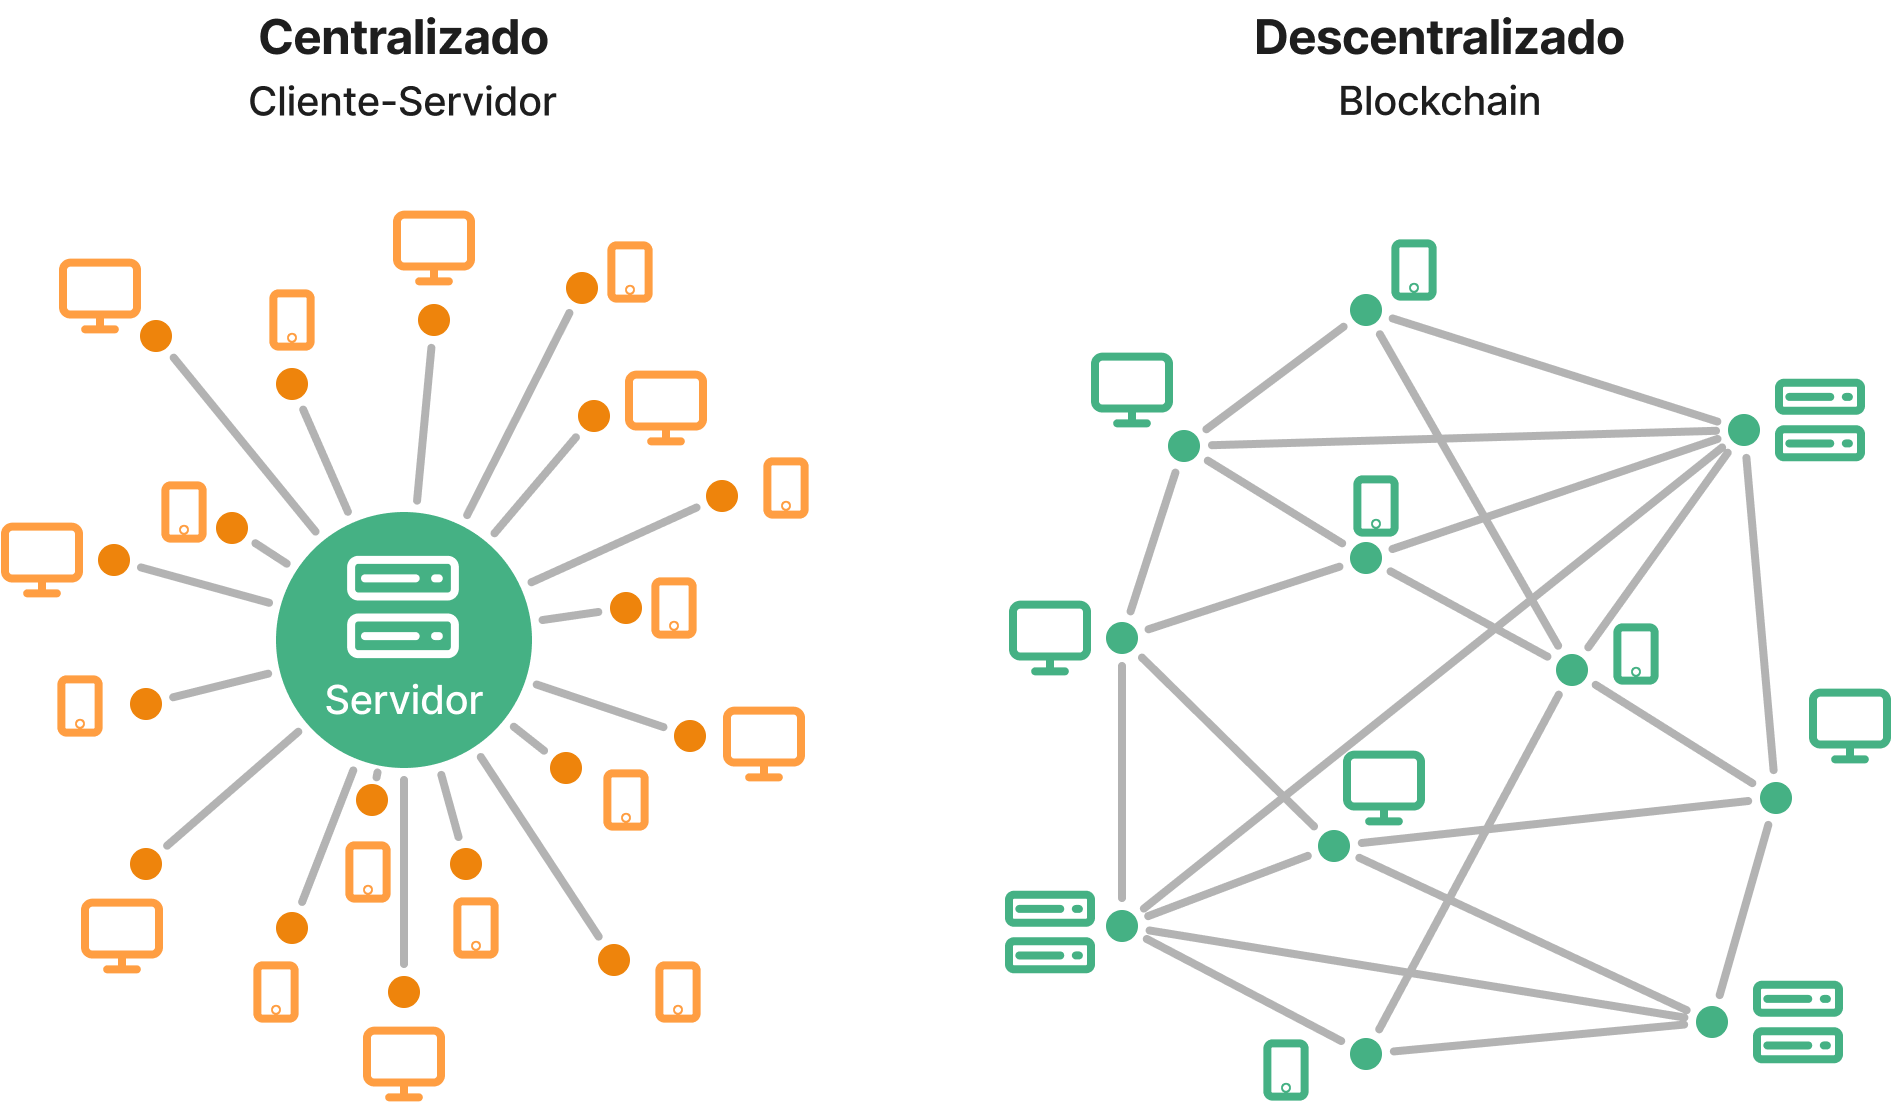
\includegraphics[width=0.8\textwidth]{Figures/client-server-vs-p2p.png}
    \caption{Comparación entre el modelo cliente-servidor y el modelo distribuido de blockchain}
    \label{fig:web-architecture}
\end{figure}

A diferencia de lo que suele suponerse, blockchain no se basa en tecnologías radicalmente nuevas, sino que integra de forma innovadora principios existentes de la computación y las matemáticas. Combina conceptos de criptografía (para asegurar la información), redes distribuidas (para la replicación de los datos) y teoría de juegos e incentivos (para coordinar el comportamiento de los participantes y garantizar la seguridad de los datos) \cite{sunny2022systematic, bulkowska2023implementation}. Esta integración produce un sistema seguro, transparente y resistente a manipulaciones, características difíciles de lograr en modelos centralizados. De esta manera, blockchain impulsa un nuevo paradigma donde el registro de la información es gestionado colectivamente, lo que permite transacciones y acuerdos entre pares sin depender de un tercero de confianza centralizado.

A continuación, se explorará en detalle la estructura y funcionamiento de la tecnología blockchain, sus características distintivas, los mecanismos de consenso que garantizan su seguridad y el papel de los \glspl{contratointeligente} como herramientas para la automatización de procesos. Además, se analizarán las ventajas y oportunidades asociadas a su implementación, así como su potencial de uso más allá del ámbito financiero.

\subsection{Estructura y Funcionamiento de una Blockchain}

La tecnología \textit{\gls{blockchain}}, o cadena de bloques, es una estructura de datos distribuida y descentralizada donde la información se organiza en transacciones agrupadas en bloques enlazados criptográficamente. Cada bloque posee un código único, conocido como \textit{\gls{hash} del bloque}, que lo identifica y sirve para enlazarlo al bloque posterior. El hash de cada bloque se genera a partir de su contenido y del hash del bloque anterior, creando así una cadena continua de bloques interconectados \cite{tripathi2023comprehensive}. En la Figura \ref{fig:blockchain-basic} se ilustra la estructura simplificada de una blockchain, donde cada bloque incluye el hash del bloque anterior, formando una cadena de bloques interconectados.

\begin{figure}[!ht]
    \centering
    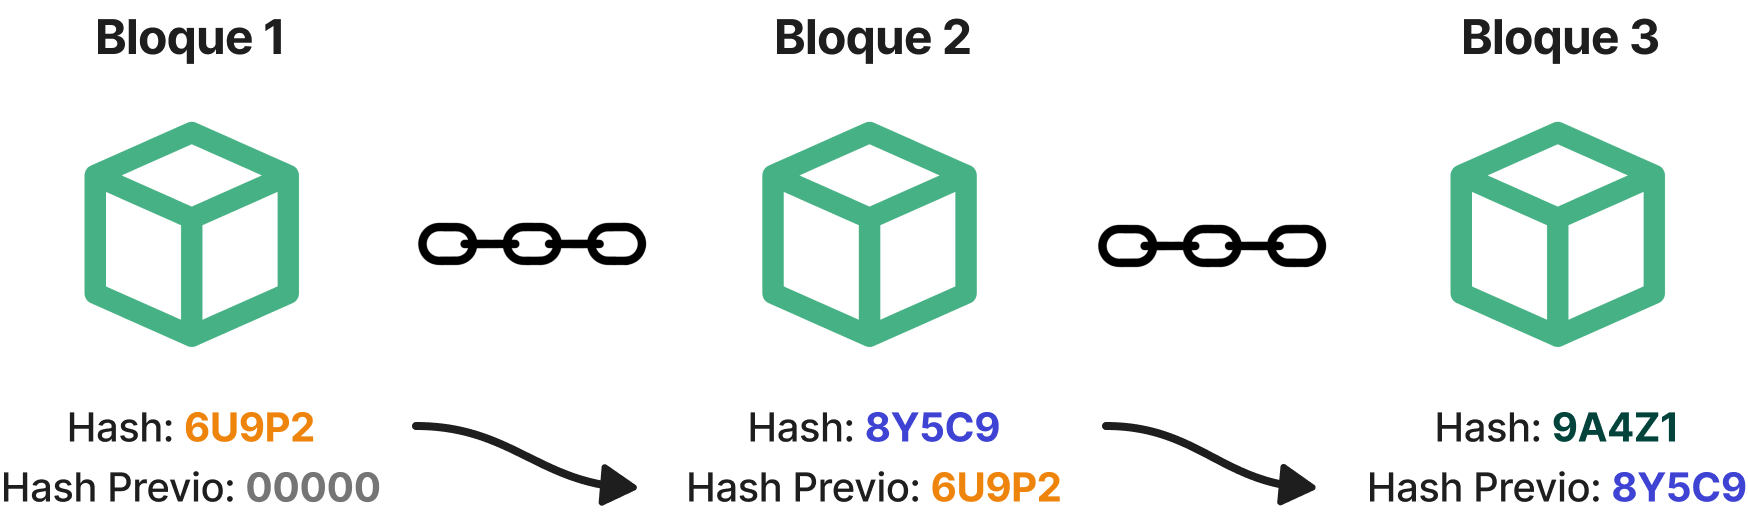
\includegraphics[width=0.8\textwidth]{Figures/blockchain-basic.png}
    \caption{Estructura básica de una cadena de bloques}
    \label{fig:blockchain-basic}
\end{figure}

Cada bloque de la cadena consta de un encabezado y un cuerpo \cite{tripathi2023comprehensive}. El cuerpo guarda la lista de transacciones, mientras que el encabezado contiene metadatos (que pueden variar en cada implementación). Entre los metadatos más relevantes se encuentran el código único del bloque anterior, una marca de tiempo y el código que identifica unívocamente al bloque actual. En la Figura \ref{fig:block-structure} se puede observar un esquema del contenido de un bloque de la cadena.

\begin{figure}[!b]
    \centering
    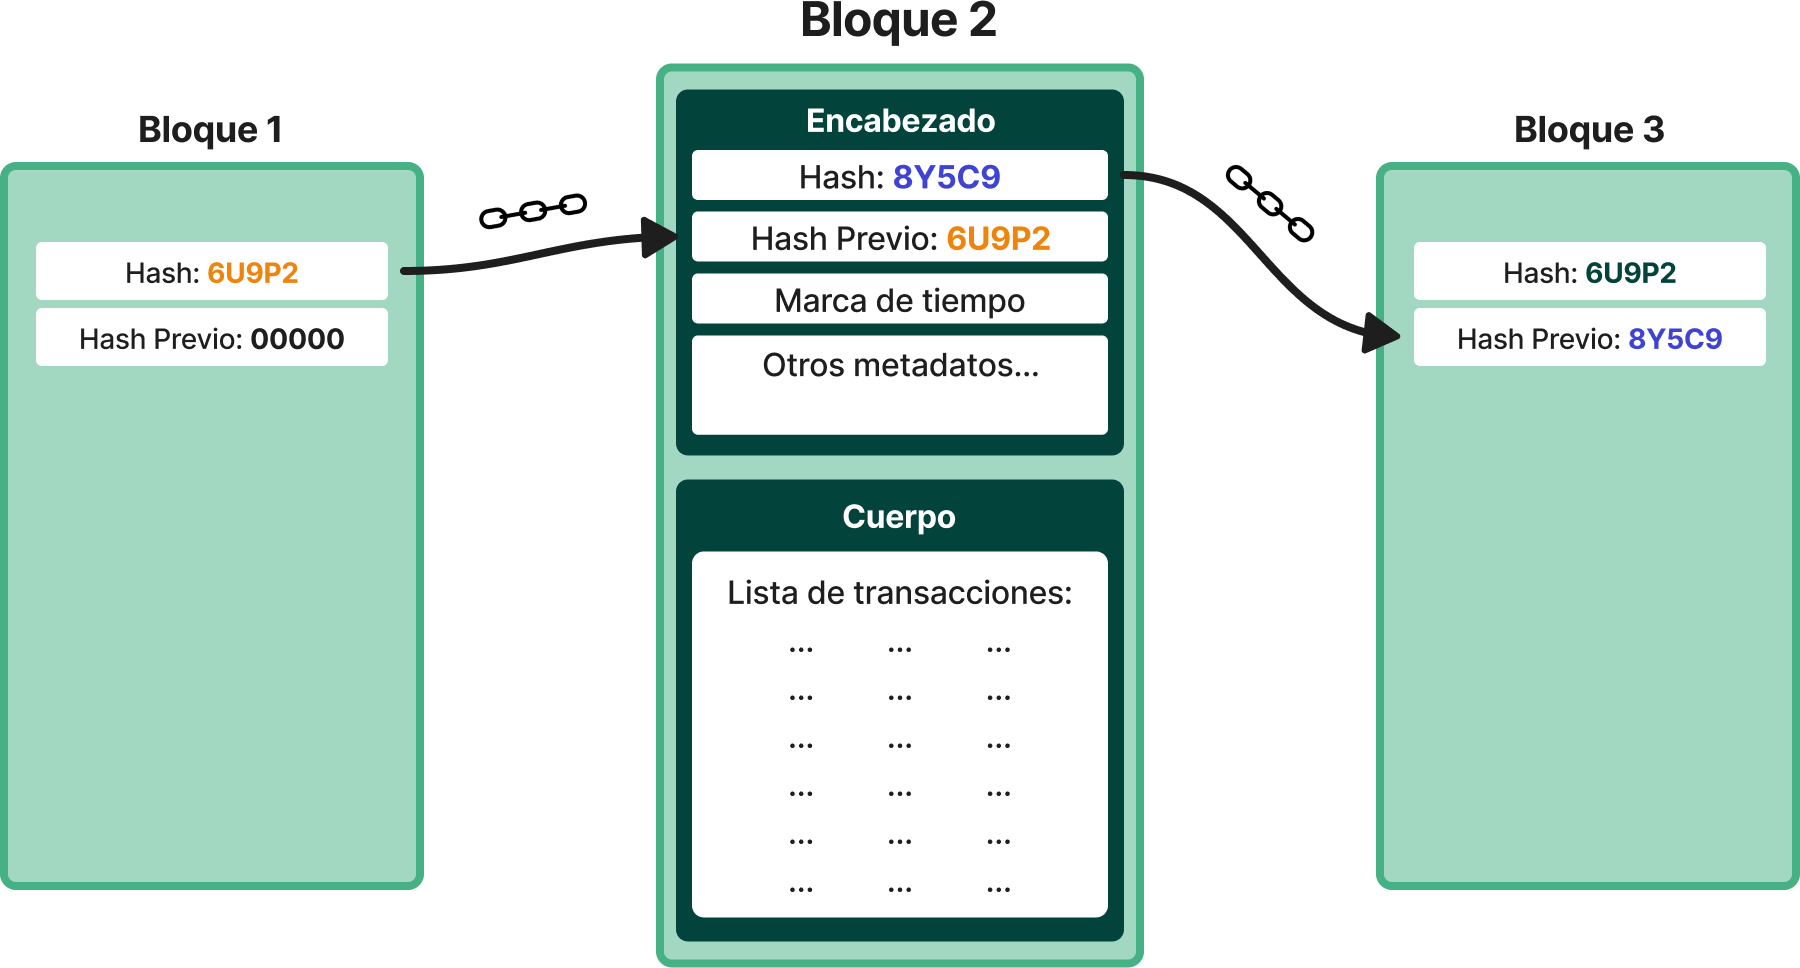
\includegraphics[width=0.8\textwidth]{Figures/block-structure.png}
    \caption{Contenido de un bloque en una cadena de bloques}
    \label{fig:block-structure}
\end{figure}

El hash del bloque se calcula usando funciones hash criptográficas, que son algoritmos matemáticos que transforman datos de entrada en una cadena de caracteres de longitud fija. Los códigos hash tienen la propiedad de ser rápidos de calcular, difíciles de revertir (es matemáticamente imposible hacerles ingeniería inversa) y únicos para cada conjunto de datos (cualquier cambio en el contenido del bloque generará un código hash completamente diferente). Estas características permiten verificar la integridad de los datos almacenados en la cadena, ya que el código hash de un bloque se puede recalcular en cualquier momento y comparar con el código almacenado en la cadena \cite{satoshi2008bitcoin}. Si los códigos coinciden, se puede confiar en que los datos no han sido alterados; si no coinciden, se ha producido una modificación no autorizada en el contenido del bloque. En la Figura \ref{fig:hash-example} se puede ver un ejemplo de los códigos generados usando un algoritmo hash a partir de dos cadenas parecidas, donde se observa que incluso un cambio mínimo en el contenido produce un hash completamente diferente. 

\begin{figure}[!tb]
    \centering
    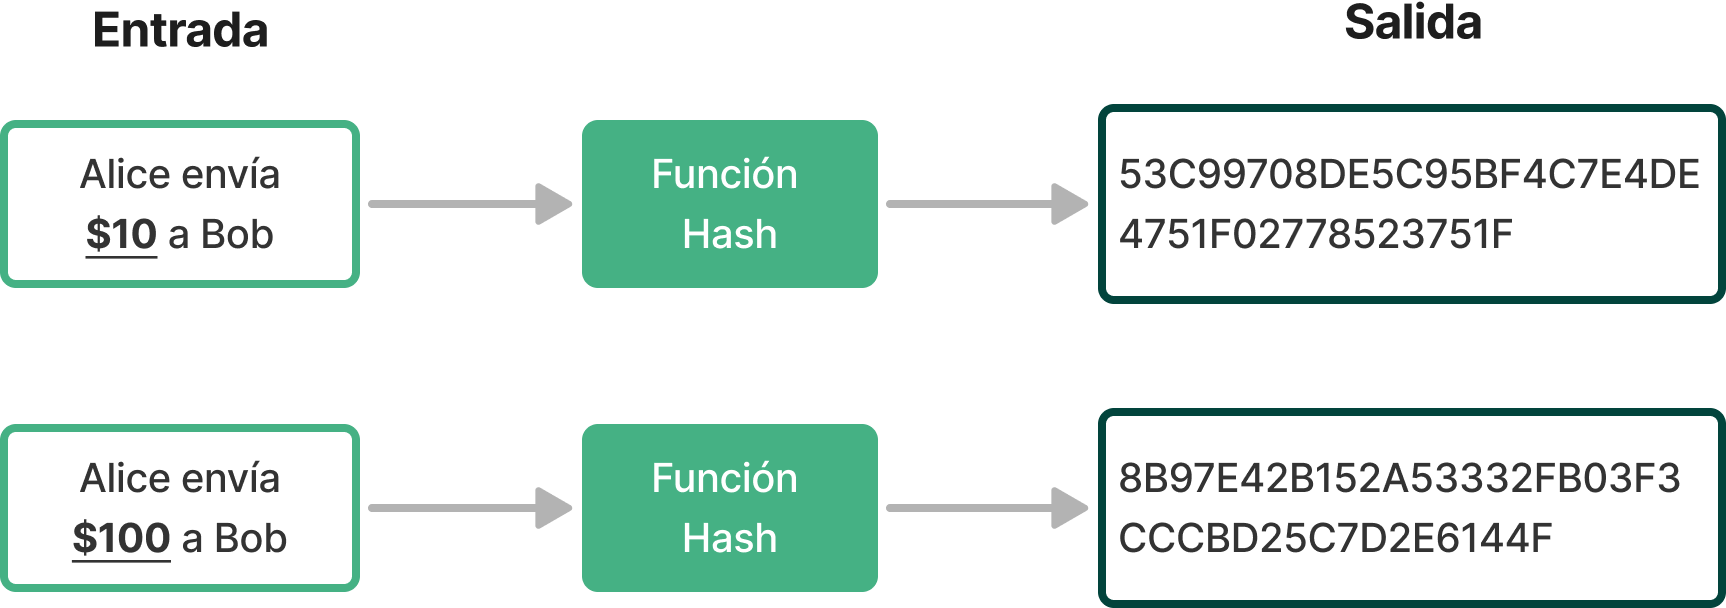
\includegraphics[width=0.8\textwidth]{Figures/hash-example.png}
    \caption{Ejemplo de códigos hash generados a partir de cadenas de texto}
    \label{fig:hash-example}
\end{figure}

La interconexión criptográfica entre los bloques confiere a blockchain su característica de inmutabilidad. Una vez que un bloque es añadido a la cadena, su hash se calcula a partir de su contenido y el hash del bloque anterior. Cualquier intento de alterar el contenido del bloque invalidaría este hash y, por ende, los hashes de todos los bloques subsiguientes, rompiendo la integridad criptográfica de la cadena. Este mecanismo permite la detección de cualquier intento de manipulación y la preservación de la integridad histórica del registro \cite{bulkowska2023implementation}. 

La naturaleza distribuida de la blockchain implica que la información no se encuentra almacenada en un único servidor, sino que está distribuida en una red de computadoras interconectadas (conocidas como nodos) y cada \gls{nodo} de la red mantiene una copia completa y actualizada del registro (de toda la cadena de bloques). Esto asegura su transparencia y resiliencia al no depender de un servidor central \cite{bulkowska2023implementation} propenso a ataques maliciosos y puntos únicos de fallo. Por su parte, la descentralización implica la ausencia de una autoridad central, de modo que la validación y adición de nuevos bloques se rigen por un \textit{\gls{mecanismodeconsenso}} entre todos los nodos participantes de la red. 

Precisamente en este marco, los mecanismos de consenso son algoritmos o una serie de reglas que se definen en una red distribuida para que todos los nodos (que en este caso deben guardar exactamente la misma cadena de bloques) se pongan de acuerdo sobre qué información es correcta y válida (Figura \ref{fig:decentralized-consensus}). Sin un mecanismo de consenso, la red sería vulnerable a ataques por parte de nodos maliciosos que puedan esparcir información inválida por la red con fines de beneficio propio, pudiendo perjudicar al resto de la red. Por ejemplo, en la red Bitcoin, cada transacción representa una transferencia de fondos entre cuentas; un nodo podría difundir transacciones al resto de la red registrando que cientos de usuarios le transfirieron fondos a una cuenta en específico, si el mecanismo de consenso no definiera reglas para validar el origen legítimo de cada transacción, este nodo malicioso podría robar los fondos de los demás usuarios para beneficio exclusivo de quien lo controla \cite{satoshi2008bitcoin}.

\begin{figure}[!htb]
    \centering
    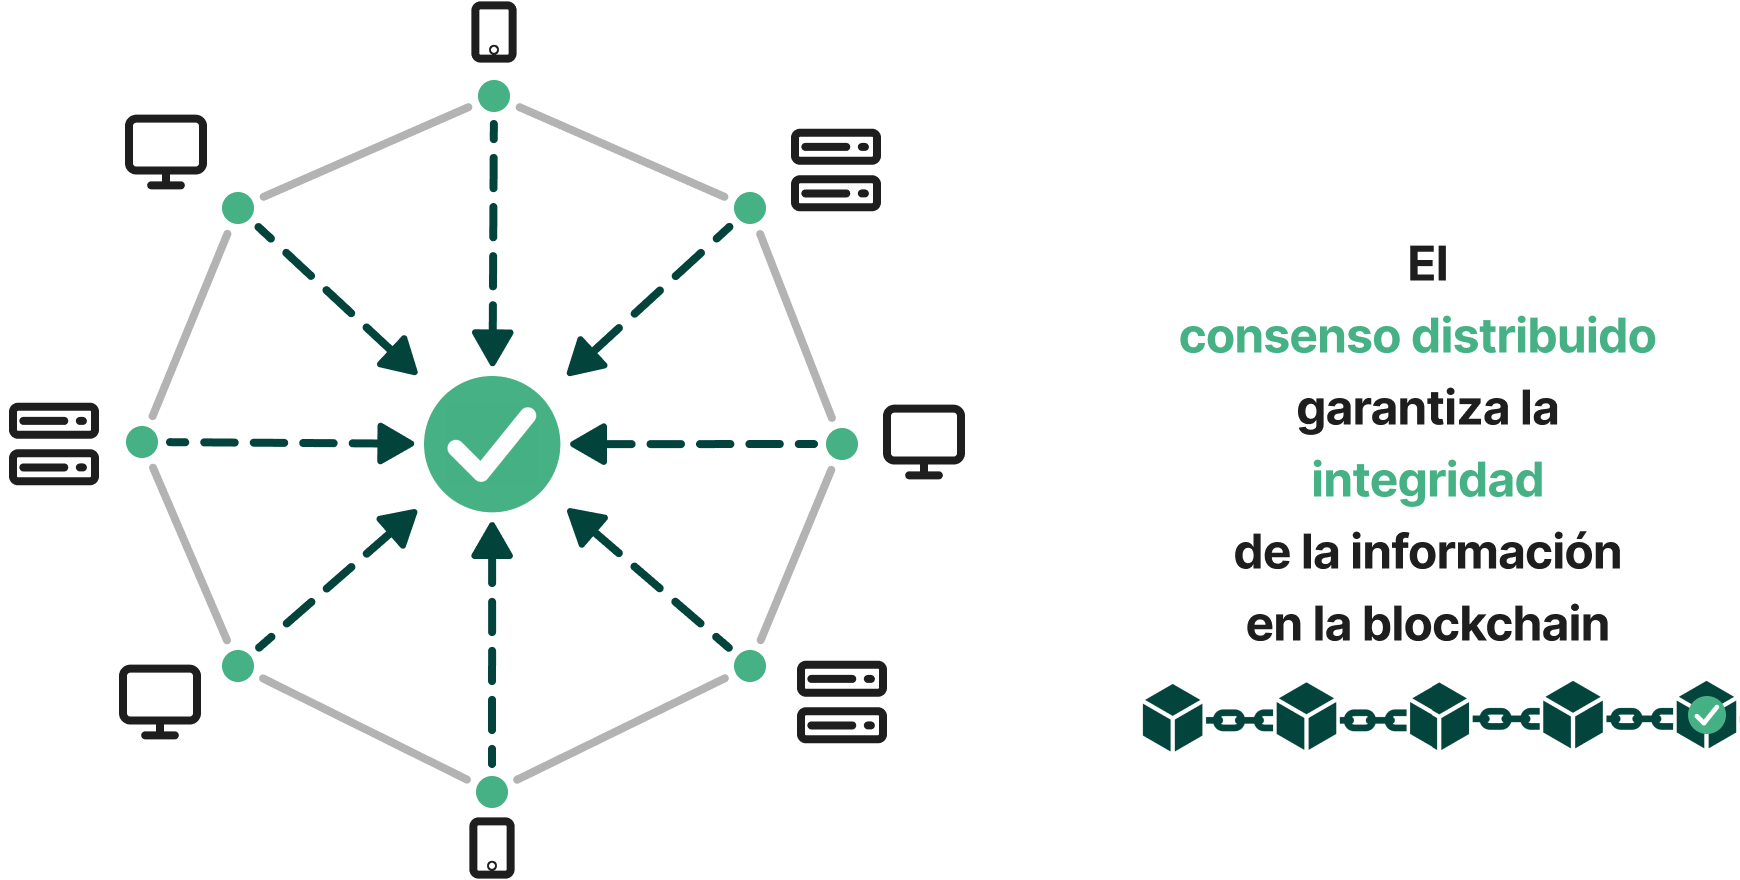
\includegraphics[width=0.8\textwidth]{Figures/decentralized-consensus.png}
    \caption{Esquema de un mecanismo de consenso en una \gls{reddescentralizada}}
    \label{fig:decentralized-consensus}
\end{figure}

Cada \gls{nodo} de la red blockchain ejecuta un mismo programa computacional (\gls{software}) que codifica las reglas del mecanismo de consenso, definiendo cómo crear transacciones y bloques válidos, transmitirlos a la red y comprobar la validez de una transacción o bloque recibido de otro nodo antes de agregarlo a su copia local de la cadena (o descartarlo si no es válido) \cite{bartolomeo2020introduccion}. Para unirse a la red, un nuevo nodo descarga una copia completa de la cadena de bloques existente, lo que le confiere una visión completa del historial de transacciones y el estado actual de la cadena \cite{bulkowska2023implementation}. Posteriormente, el nodo comienza a ejecutar el software del mecanismo de consenso. A partir de entonces, el nodo puede generar nuevas transacciones y transmitirlas a la red para ser recibidas por los demás nodos. Asimismo, el nodo recibe transacciones de otros nodos y las valida mediante el mecanismo de consenso antes de añadirlas a un bloque en su copia local de la cadena \cite{bulkowska2023implementation}.

En la actualidad, existen múltiples algoritmos de consenso que definen distintas formas de generar un bloque válido (desde un nodo) y comprobar la validez del bloque (recibido desde otro nodo). Cada \gls{mecanismodeconsenso} utiliza diferentes técnicas de teoría de juegos con el objetivo de incentivar a que se unan nuevos nodos a la red mediante recompensas y desincentivar que un nodo actúe de manera maliciosa para obtener un beneficio individual. El mecanismo de consenso garantiza que la red se mantenga segura y resistente a ataques combinando esquemas donde la penalización o pérdida generada por un comportamiento malicioso supere con creces las ganancias que se puedan obtener comportándose de forma maliciosa \cite{satoshi2008bitcoin}. Ejemplos prominentes de la diversidad de mecanismos incluyen la Prueba de Trabajo (\acrshort{pow}), la Prueba de Participación (\acrshort{pos}) y la Prueba de Autoridad (\acrshort{poa}), cada uno con características particulares.

El mecanismo de Prueba de Trabajo (\acrshort{pow}, por sus siglas en inglés) es uno de los algoritmos de consenso más conocidos y el primero introducido en las redes blockchain por su implementación en Bitcoin \cite{satoshi2008bitcoin}. En \acrshort{pow}, todos los nodos (conocidos como ``mineros'' en este contexto) compiten para resolver un problema matemático complejo que requiere una gran capacidad computacional. El primer nodo que logra resolver este problema matemático valida la transacción y crea el nuevo bloque incluyendo la solución en su encabezado. El resto de nodos recibe el bloque y comprueba que el problema haya sido resuelto correctamente. El nodo que resuelve el reto recibe una compensación en Bitcoin como incentivo por aportar un bloque válido a la red. Aunque la validación de un bloque es de complejidad constante, la alteración de un bloque ya existente implicaría la necesidad de recalcular no solo dicho bloque, sino también todos los bloques subsiguientes. Esto convierte la modificación en un proceso extremadamente costoso en términos de recursos computacionales y energía, lo cual, sumado al rechazo de la red hacia cualquier cadena alterada, desincentiva eficazmente los intentos de manipulación \cite{satoshi2008bitcoin}. La desventaja de este algoritmo de consenso es que implica un alto costo energético debido a la carga computacional requerida para resolver el problema \cite{diez2023web}.

Otro mecanismo ampliamente utilizado es la Prueba de Participación (\acrshort{pos}, por sus siglas en inglés), a diferencia de \acrshort{pow}, no requiere de una alta capacidad computacional para la creación de bloques. En \acrshort{pos}, los \glspl{nodo} (conocidos como validadores) ``apuestan'' una cantidad de \glspl{criptomoneda} como garantía de su buen comportamiento. Para generar un bloque válido, el protocolo selecciona pseudo-aleatoriamente un validador para generar el siguiente bloque, con una probabilidad de selección proporcional a la cantidad de criptomonedas que ha apostado. Una vez que el validador seleccionado crea un bloque y lo transmite a la red, los demás nodos validadores de la red simplemente comprueban que el bloque cumpla con las reglas de negocio del protocolo. Si un validador actúa de manera maliciosa, puede perder parte o la totalidad de su participación (proceso conocido como ``slashing''). La principal ventaja del \acrshort{pos} es su eficiencia energética significativamente mayor en comparación con \acrshort{pow}, ya que no se requiere una minería intensiva. Además, puede ofrecer mayor escalabilidad y tarifas de transacción más bajas. Ethereum es un ejemplo de protocolo blockchain que fue implementado originalmente con \acrshort{pow}, pero que se actualizó para utilizar \acrshort{pos} debido a estas ventajas. Sin embargo, una desventaja potencial es el riesgo de centralización si la mayoría de la participación se acumula en pocos nodos, lo que podría darles un control desproporcionado sobre la red \cite{tripathi2023comprehensive}.

La Prueba de Autoridad (\acrshort{poa}, por sus siglas en inglés) es otro mecanismo de consenso donde la validación de bloques se basa en la identidad y reputación de un conjunto pre-aprobado de validadores. Para generar un bloque válido, el protocolo elige una autoridad designada (del conjunto de validadores aprobados y de confianza) que tiene el derecho exclusivo de crear y firmar el nuevo bloque. Para verificar que un bloque es válido, los demás nodos de la red simplemente comprueban la firma digital del validador que lo propuso y que el bloque cumple con las reglas del protocolo. La principal ventaja del \acrshort{poa} es su alta velocidad de transacción, ya que solo un número limitado de validadores de confianza necesita llegar a un consenso. Esto lo hace ideal para redes privadas o consorcios donde la confianza entre los participantes ya existe. Sin embargo, esta misma es su mayor desventaja, ya que la seguridad y el control de la red dependen de un pequeño grupo de entidades conocidas, lo que va en contra del principio de descentralización de muchas blockchains públicas \cite{diaz2022protocolos}.

Cada uno de los mecanismos mencionados ofrece distintos niveles de eficiencia de procesamiento, seguridad y descentralización. Durante la validación del bloque, se verifican múltiples aspectos en común en cualquiera de estos mecanismos: la correcta correspondencia del hash del bloque anterior con el almacenado en el encabezado del nuevo bloque, la validez de las transacciones de acuerdo a la lógica de negocios propia del protocolo blockchain, y que el hash del bloque propuesto haya sido generado correctamente a partir de la totalidad de su contenido.

En síntesis, la robustez de una blockchain reside en la interconexión sinérgica de sus componentes: el encadenamiento criptográfico, la red distribuida y el \gls{mecanismodeconsenso}. No es un único elemento el que garantiza su seguridad e integridad, sino la forma en que estos principios interactúan constantemente. Los mecanismos de consenso, en particular, son los encargados de arbitrar la creación de nuevos bloques de forma segura, resolviendo el problema de la confianza en un entorno descentralizado. A su vez, el encadenamiento criptográfico asegura la inmutabilidad de la información, ya que cualquier alteración maliciosa en un bloque de la cadena modificaría su hash y rompería la consistencia posterior de la cadena, forzando a cada nodo de la \gls{reddescentralizada} a rechazar el bloque modificado. En consecuencia, para recuperar la consistencia de la cadena, sería necesario modificar los hashes de todos los bloques posteriores, lo que sería un proceso computacionalmente costoso y fácilmente detectable por el resto de la red. 

A través de un proceso iterativo de validación, los \glspl{nodo} de la red trabajan de forma coordinada para generar, verificar y distribuir nuevos bloques, conformando un ciclo de vida que asegura la consistencia y la inmutabilidad de la cadena de bloques \cite{bartolomeo2020introduccion}. Luego de conocer los elementos fundamentales que conforman una blockchain, es posible analizar cómo interactúan para registrar y validar transacciones de manera coordinada en un entorno descentralizado. El proceso se desarrolla de forma secuencial y repetitiva, asegurando que cada bloque añadido a la cadena preserve la integridad del registro global de transacciones. En la Figura \ref{fig:blockchain-working} se presenta un esquema ilustrativo con los pasos del proceso de incorporación de una nueva transacción y su respectivo bloque en una blockchain. A continuación, se describen estos pasos en detalle:

\begin{figure}[!tb]
    \centering
    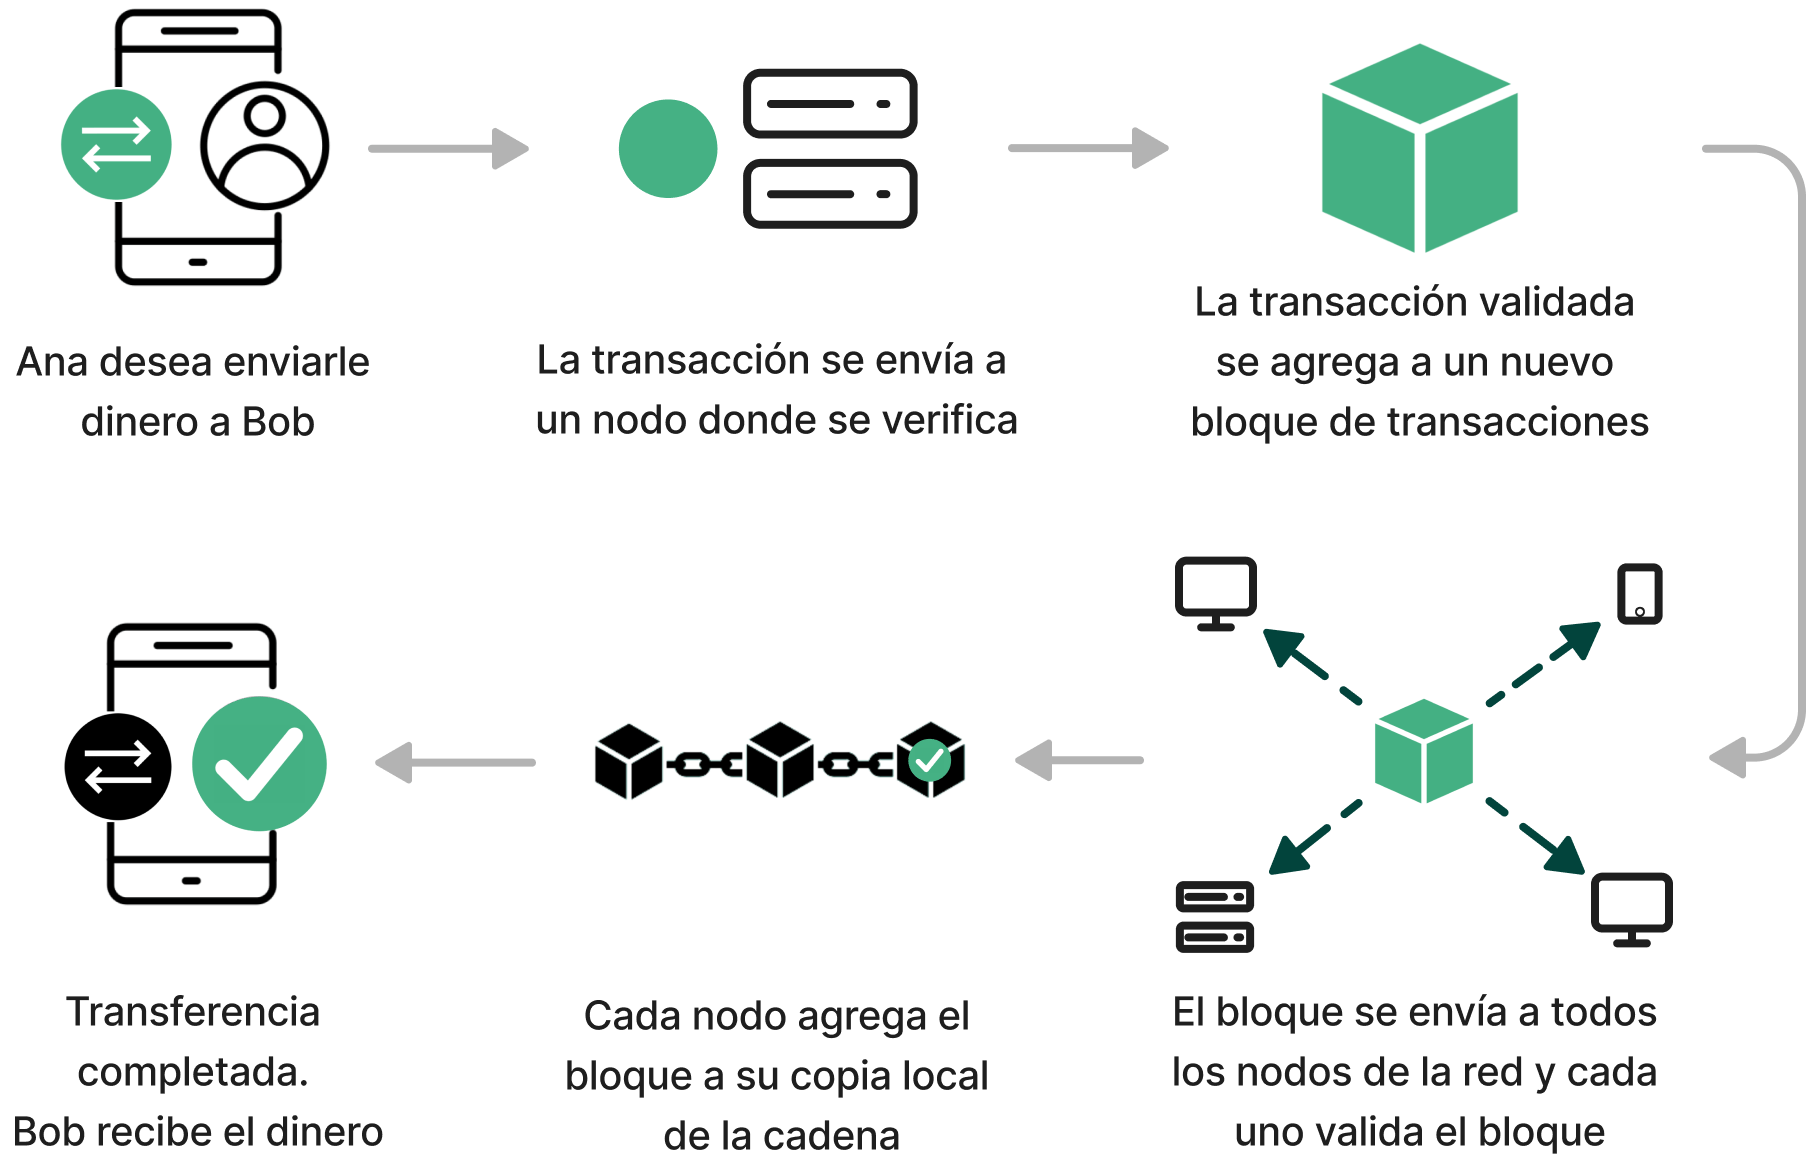
\includegraphics[width=\textwidth]{Figures/block-creation.png}
    \caption{Proceso de creación de una transacción y un bloque en una blockchain}
    \label{fig:blockchain-working}
\end{figure}

\begin{enumerate}
    \item Un \gls{nodo} de la red crea y firma una nueva transacción con su clave privada (la firma criptográfica garantiza la autenticidad de la transacción).
    \item La transacción se propaga a través de la red distribuida, donde es recibida por cada nodo participante.
    \item Cada nodo valida la transacción individualmente, verificando la firma del remitente y asegurándose de que la transacción cumple con la lógica de negocios propia del protocolo blockchain (por ejemplo, en Bitcoin, que el remitente cuente con los fondos a transferir). Una vez validada, la transacción se añade a un \textit{pool} de transacciones pendientes. En caso de ser inválida, simplemente se ignora y se descarta. 
    \item Cuando un nodo tiene suficiente cantidad de transacciones en su \textit{pool}, procede a seleccionar un conjunto de transacciones pendientes del \textit{pool} para formar un nuevo bloque. Este bloque incluye las transacciones seleccionadas, el hash del bloque anterior y otros metadatos (como la marca de tiempo y un \textit{nonce} para \acrshort{pow}). Luego, el nodo calcula el hash de este nuevo bloque y, según el algoritmo de consenso, realiza el trabajo necesario para garantizar que sea válido. En el caso de \acrshort{pow}, esto implica resolver un problema criptográfico que requiere una cantidad significativa de potencia computacional. En \acrshort{pos}, el nodo debe demostrar que posee una cantidad suficiente de fondos para participar en la validación del bloque.
    \item Una vez que el nodo ha validado el nuevo bloque (o ``minado'' en \acrshort{pow}), lo difunde a la red. Los demás nodos reciben este bloque y verifican su validez (incluyendo el hash, las transacciones y la prueba de trabajo/participación). Si el bloque es válido, cada nodo lo añade a su copia local de la cadena de bloques y descarta de su \textit{pool} de pendientes las transacciones incluidas en el bloque. Si el bloque es inválido, es rechazado por cada nodo y no se añade a la cadena.
\end{enumerate}

De esta manera, la cadena de bloques se actualiza de forma continua y descentralizada, asegurando que todos los nodos de la red mantengan una copia idéntica y consistente del registro de transacciones \cite{bartolomeo2020introduccion}. En su concepción inicial, las transacciones en un bloque se asociaban comúnmente a movimientos financieros \cite{satoshi2008bitcoin}, pero la flexibilidad inherente de la tecnología blockchain permite que los bloques contengan cualquier tipo de información estructurada \cite{bartolomeo2020introduccion}. Esta versatilidad ha sido el motor para el desarrollo de aplicaciones más complejas, destacando entre ellas los contratos inteligentes \cite{sunny2022systematic}, que permiten almacenar programas computacionales en la blockchain, habilitando la automatización segura de procesos como la trazabilidad, la certificación de origen o la valorización de materiales reciclados.

\subsection{Contratos Inteligentes}
\label{sec:smart-contracts}

A mediados de la década de 1990, cuando el comercio electrónico comenzaba a expandirse y se buscaban mecanismos seguros para realizar transacciones entre personas sin relación previa y sin confianza mutua, el criptógrafo y jurista Nick Szabo propuso el concepto de \gls{contratointeligente} \cite{buterin2013ethereum}. Lo definió como un protocolo informático diseñado para ejecutar de forma automática los términos de un acuerdo, reduciendo la necesidad de intermediarios humanos y de documentos legales tradicionales.

En su concepción original, estos contratos no dependían necesariamente de blockchain. Sin embargo, la aparición de esta tecnología a partir de Bitcoin en 2008 y, especialmente, la introducción de Ethereum en 2015, proporcionó por primera vez una infraestructura distribuida, segura e inmutable capaz de materializar la idea de Szabo. Actualmente, un contrato inteligente es un programa almacenado en una blockchain que se activa y ejecuta automáticamente cuando se cumplen condiciones predefinidas, garantizando que los acuerdos se lleven a cabo tal como fueron codificados, sin intervención de terceros de confianza \cite{bulkowska2023implementation}. Su función principal es automatizar procesos en entornos descentralizados, reduciendo la dependencia de intermediarios humanos \cite{verma2023overview} y mejorando la eficiencia operativa en múltiples sectores \cite{sunny2022systematic}.

Para codificar las reglas de un contrato inteligente, se emplean lenguajes de programación específicos adaptados a cada plataforma blockchain \cite{bartolomeo2020introduccion}. Un ejemplo prominente es \textit{Solidity} \cite{taherdoost2023smart}, utilizado en Ethereum, un lenguaje orientado a objetos diseñado específicamente para esta finalidad. Los contratos programados en Solidity pueden interactuar entre sí y con el estado global de la blockchain, habilitando la creación de aplicaciones descentralizadas (conocidas también como \acrshort{dapps}, por sus siglas en inglés) que operan de forma autónoma y sin intermediarios en la red \cite{buterin2013ethereum}.

Un contrato inteligente se concibe como un conjunto de reglas y lógica de negocio codificadas. Cada contrato posee un código (las reglas, por ejemplo, en Solidity) y un estado (la información dinámica almacenada en la blockchain) \cite{buterin2013ethereum}. El código del contrato es inmutable una vez desplegado en la blockchain mediante una transacción, garantizando la permanencia de las reglas establecidas. Su estado, sin embargo, puede evolucionar a medida que se interactúa con el contrato a través de transacciones. Es importante destacar que, si bien se describen como auto-ejecutables por su automatismo al cumplir condiciones, su ejecución es llevada a cabo por los \glspl{nodo} de la red que validan las transacciones e integran los cambios de estado en la cadena \cite{buterin2013ethereum}. Tanto el código como el estado del contrato se almacenan en la blockchain, asegurando su transparencia y disponibilidad pública. Por ejemplo, un contrato inteligente podría gestionar un sistema de votación, donde los participantes envían sus votos y el contrato contabiliza automáticamente los resultados al finalizar el periodo de votación. En la Figura \ref{fig:smart-contract-process} se ilustra el proceso de definición y utilización de un contrato inteligente en una blockchain.

\begin{figure}[!tb]
    \centering
    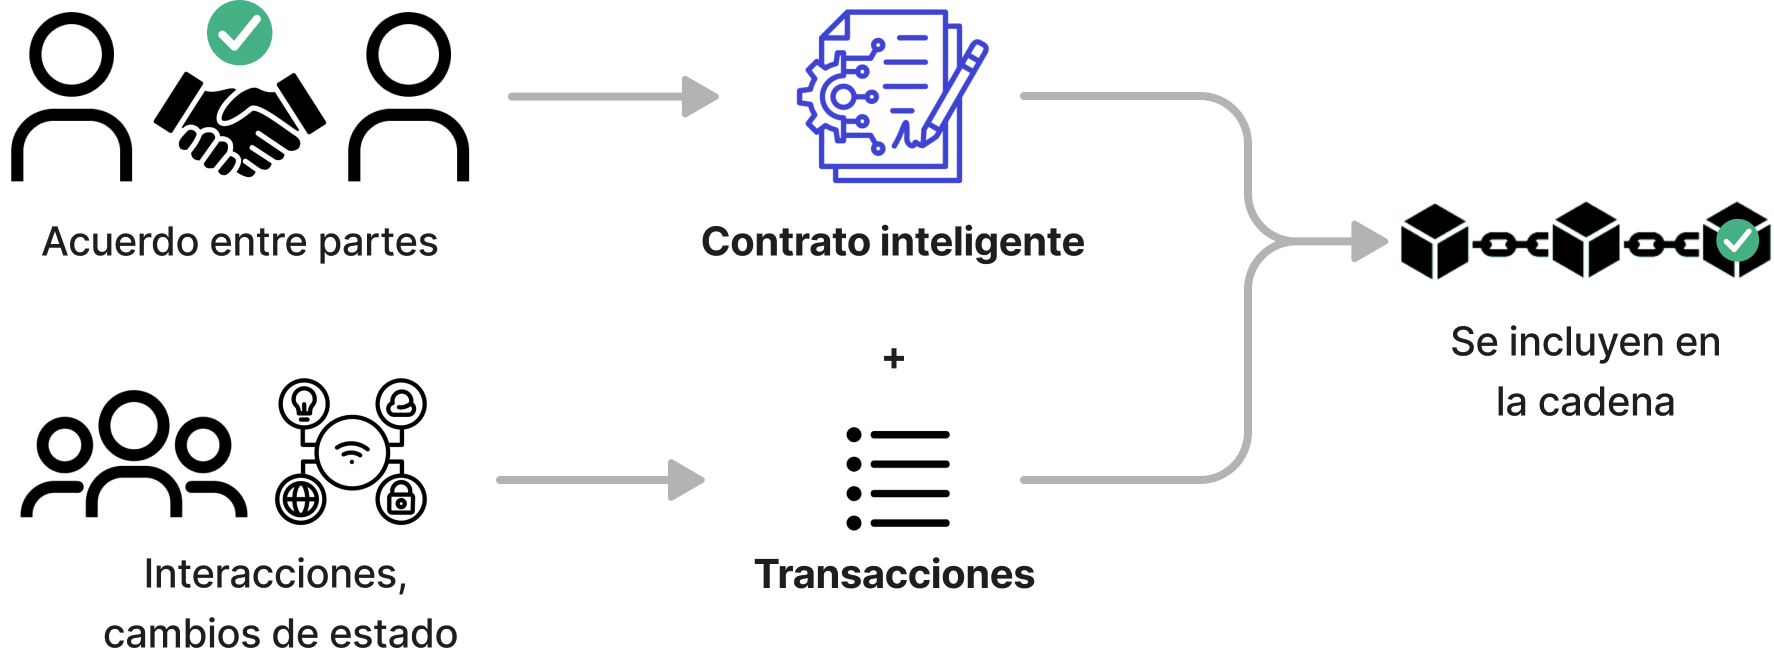
\includegraphics[width=0.9\textwidth]{Figures/smart-contract-process.png}
    \caption{Ciclo de vida de un contrato inteligente}
    \label{fig:smart-contract-process}
\end{figure}

Además de las ventajas generales de la tecnología blockchain, los contratos inteligentes aportan beneficios y desafíos específicos frente a la automatización de procesos basada en sistemas digitales tradicionales. Entre sus principales ventajas, destacan la capacidad de ejecutar acuerdos de forma automática y verificable sin necesidad de intermediarios, la transparencia y auditabilidad del código y de su historial de transacciones, así como la posibilidad de integrarse con otros contratos para crear procesos más complejos \cite{bartolomeo2020introduccion}. Estas propiedades permiten reducir fricciones operativas, agilizar procesos y ofrecer garantías criptográficas de que las reglas se cumplen tal como fueron definidas.

Sin embargo, los contratos inteligentes enfrentan limitaciones inherentes a las infraestructuras blockchain, principalmente en términos de escalabilidad \cite{kalajdjieski2023databases}. A diferencia de los sistemas centralizados que permiten ejecución paralela y optimización con bases de datos indexadas, los contratos inteligentes operan bajo modelos de ejecución secuencial y replicación completa en cada nodo \cite{taherdoost2023smart}. Esto impacta directamente su rendimiento y complejiza la implementación de algoritmos avanzados. Desde la perspectiva de la \gls{ingenieriadesoftware}, el desarrollo de contratos inteligentes introduce restricciones no triviales: el código inmutable, los costos asociados al almacenamiento en cadena, la ausencia de llamadas externas directas y los modelos de estado global distribuido. Estas particularidades exigen la adopción de nuevas metodologías y prácticas de diseño seguro, control de flujos y validación estática, muchas de las cuales aún se encuentran en proceso de estandarización \cite{taherdoost2023smart, cepal2021economia}.

En síntesis, los contratos inteligentes constituyen una herramienta computacional que expande las fronteras de la programación distribuida y descentralizada. Si bien su potencial transformador es innegable \cite{taherdoost2023smart}, su desarrollo robusto y seguro representa un desafío activo que abarca múltiples dominios de la computación: desde la teoría de lenguajes formales \cite{hoskinson2017we} y la arquitectura de sistemas distribuidos, hasta la verificación de software, la criptografía aplicada y la integración de datos externos confiables \cite{taherdoost2023smart}. Debido a la aparición de los contratos inteligentes, la tecnología blockchain ha trascendido su origen ligado a las \glspl{criptomoneda} para convertirse en un paradigma disruptivo con aplicaciones transversales en múltiples dominios \cite{bartolomeo2020introduccion, vaigandla2023review}. En la actualidad, los contratos inteligentes se posicionan como un componente fundamental y un impulsor clave de gran parte de las nuevas y complejas soluciones basadas en blockchain, especialmente aquellas que buscan automatizar procesos y gestionar la lógica de negocio directamente en la cadena \cite{sharabati2024blockchain}. Si bien representan una tecnología prometedora, aún se encuentran en una etapa incipiente, lo que implica la existencia de numerosos aspectos por perfeccionar \cite{taherdoost2023smart}. En un contexto más amplio, la tecnología blockchain, incluyendo a los contratos inteligentes, ofrece una serie de ventajas fundamentales y limitaciones inherentes que la distinguen de los sistemas de almacenamiento de datos tradicionales.

\subsection{Desafíos y Oportunidades}

Las características inherentes de la blockchain, detalladas previamente, se traducen en una serie de ventajas que la distinguen de tecnologías tradicionales. La descentralización propia de su diseño y la consecuente eliminación de intermediarios resultan en una mayor confianza \cite{rejeb2023role} y eficiencia operativa al prescindir de autoridades centrales \cite{sharabati2024blockchain}. La arquitectura basada en registros inmutables garantiza transparencia y \gls{trazabilidad} completa \cite{sharabati2024blockchain}, permitiendo un historial verificable de cualquier activo o evento, lo cual es crucial para casos de uso como certificación \cite{bartolomeo2020introduccion}, logística \cite{bartolomeo2020introduccion, rejeb2023role} y gestión de residuos \cite{bulkowska2023implementation}. Además, la capacidad de automatización de aplicaciones mediante \glspl{contratointeligente} optimiza la eficiencia y confiabilidad operativa al ejecutar condiciones lógicas de forma autónoma \cite{bartolomeo2020introduccion}. En conjunto, las propiedades de transparencia, inmutabilidad y seguridad confieren a blockchain una aplicabilidad transversal que la consolida como una tecnología habilitadora para la transformación digital en sectores diversos como finanzas, salud, \acrshort{iot}, energía, educación y ciudades inteligentes, entre otros.

Sin embargo, a pesar de sus beneficios, la tecnología blockchain también enfrenta desafíos y limitaciones como lo son la escalabilidad y el rendimiento \cite{tripathi2023comprehensive}. Las blockchains actuales suelen presentar un bajo rendimiento en procesamiento de información en comparación con los sistemas centralizados \cite{baralla2023waste}, debido a la necesidad de alcanzar un consenso distribuido entre todos los \glspl{nodo} de la red \cite{tripathi2023comprehensive}. Además, existen vulnerabilidades técnicas inherentes a la tecnología, como el ataque del 51\%, el doble gasto y la posibilidad de errores en contratos inteligentes mal programados, que requieren atención constante \cite{diez2023web}. La irreversibilidad de las transacciones, si bien es una garantía de seguridad, puede ser problemática ante vulnerabilidades de programación, errores o fraudes, ya que las operaciones registradas no pueden deshacerse \cite{taherdoost2023smart}. Actualmente, estos desafíos están siendo abordados activamente por la investigación y el desarrollo en la comunidad blockchain. La constante evolución de la tecnología y la aparición de nuevas soluciones buscan mitigar estas limitaciones, abriendo el camino para una adopción más amplia \cite{tripathi2023comprehensive, baralla2023waste, taherdoost2023smart}. En este contexto de evolución, la tecnología blockchain ha demostrado su potencial para transformar diversos sectores y abarcar numerosos casos de uso.

% \subsection{Casos de Uso}

En el sector financiero, blockchain ha generado disrupción mediante soluciones para pagos directos (con las llamadas \glspl{criptomoneda}) y transferencias internacionales \cite{bartolomeo2020introduccion}. A nivel gubernamental, blockchain permite la \gls{trazabilidad} de procesos administrativos, y la implementación de sistemas de votación transparentes \cite{vaigandla2023review}. En el ámbito de la salud, blockchain permite almacenar registros médicos de manera segura y distribuida, mejorando la interoperabilidad entre instituciones y permitiendo a los pacientes un mayor control de su historial médico \cite{sunny2022systematic}. Esta tecnología también se utiliza en la trazabilidad de la cadena de suministro farmacéutica, donde se requiere un alto nivel de confianza y se debe garantizar el cumplimiento normativo \cite{vaigandla2023review}. En otros rubros, como la educación, esta tecnología se utiliza para la emisión y verificación de certificados académicos digitales. A su vez, también se está utilizando blockchain para crear mercados para el comercio de energía entre pares, mejorando la gestión de certificados de energías renovables y optimizando la trazabilidad de la producción y el consumo energético \cite{sunny2022systematic, vaigandla2023review}.

En el ámbito de la gestión de la \gls{cadenadesuministro}, blockchain proporciona una plataforma confiable para garantizar la trazabilidad, autenticidad y visibilidad en tiempo real de productos y materiales \cite{torres2022tendencias, sharabati2024blockchain}. Empresas como IBM, Maersk y FedEx han implementado soluciones blockchain para monitorear inventarios, registrar pagos y reducir disputas logísticas \cite{tripathi2023comprehensive}. Otro caso ejemplar es Dervinsa en Argentina, que certifica la calidad de productos derivados de residuos de vinificación, y otras iniciativas que aplican trazabilidad a alimentos y textiles \cite{bartolomeo2020introduccion}. Dentro de modelos de \gls{economiacircular}, blockchain se posiciona como un facilitador para monitorear ciclos de vida de productos y materiales \cite{bulkowska2023implementation, baralla2023waste}. Diversos tipos de residuos, desde plásticos y vidrio hasta electrónicos y biomédicos, pueden ser gestionados de manera más eficiente mediante el uso de \glspl{contratointeligente} que automatizan verificaciones e interacciones entre actores de la cadena \cite{baralla2023waste}. Asimismo, han surgido propuestas innovadoras como la generación de pasaportes digitales de productos y esquemas de incentivos sostenibles, promoviendo hábitos de consumo responsables y nuevos modelos de negocio circulares \cite{baralla2023waste}.

La necesidad de trazar el flujo de materiales, certificar la autenticidad de los procesos productivos y garantizar la gestión responsable de residuos ha posicionado a blockchain como una herramienta protagónica para habilitar modelos circulares sostenibles. En particular, su capacidad para registrar datos inmutables y automatizar interacciones mediante contratos inteligentes permite estructurar sistemas de trazabilidad que mejoran la eficiencia operativa y también fortalecen la confianza entre actores \cite{sharabati2024blockchain, rejeb2023role}. A continuación, se analizará con mayor profundidad el uso de blockchain para trazabilidad de materiales en la cadena de suministro y para la implementación de estrategias de economía circular.

\section{Economía Circular}
\label{sec:circular-economy}

La \gls{economiacircular} es un enfoque alternativo al modelo económico lineal tradicional, que nace con el objetivo de transformar de manera sostenible la forma en que la sociedad produce, consume y gestiona los recursos naturales \cite{espanacircular2030}.

Desde la Revolución Industrial, la economía global ha operado principalmente bajo un modelo lineal de ``extraer, producir y consumir'', caracterizado por la explotación de recursos naturales y la generación masiva de residuos \cite{cerda2016economia}. En este modelo económico, los recursos son extraídos de la naturaleza, transformados en productos, consumidos y finalmente desechados al terminar su vida útil. Este enfoque, aunque ha impulsado un crecimiento económico mundial sin precedentes, ha generado sobreexplotación y degradación de ecosistemas. La deforestación, pérdida de biodiversidad, contaminación del agua, generación masiva de residuos y escasez de recursos no renovables son algunas de las consecuencias negativas de este enfoque extractivo a gran escala. A medida que la población mundial y la demanda de recursos continúan creciendo, la insostenibilidad de este modelo a largo plazo se hace cada vez más evidente \cite{clima2022book}. En el enfoque lineal, la \gls{cadenadesuministro} de materiales se organiza como un proceso unidireccional: los recursos son extraídos, transformados en productos, consumidos y finalmente desechados. Este modelo ignora el valor residual de los materiales, no contempla mecanismos para reincorporar los productos al ciclo productivo una vez finalizada su vida útil y, en consecuencia, genera una creciente acumulación de residuos. En contraste, la economía circular redefine el papel de la cadena de suministro, transformándola en una red cerrada y regenerativa. Con este enfoque, la cadena se vuelve más dinámica e interdependiente, integrando bucles de retroalimentación entre los diferentes actores de la cadena de valor, incluyendo a consumidores, productores, proveedores y gestores de residuos. El modelo circular propone un sistema en el que los recursos se mantienen en uso durante el mayor tiempo posible, se reciclan y se reutilizan, minimizando la generación de residuos y reduciendo la extracción de materias primas \cite{ellenmacarthurfoundation2022}. La diferencia estructural entre la economía lineal y la economía circular se hace evidente al ilustrar el flujo de recursos en ambos modelos, como se muestra en la Figura \ref{fig:circular-linear-economy-comparison}.

\begin{figure}[!tb]
    \centering
    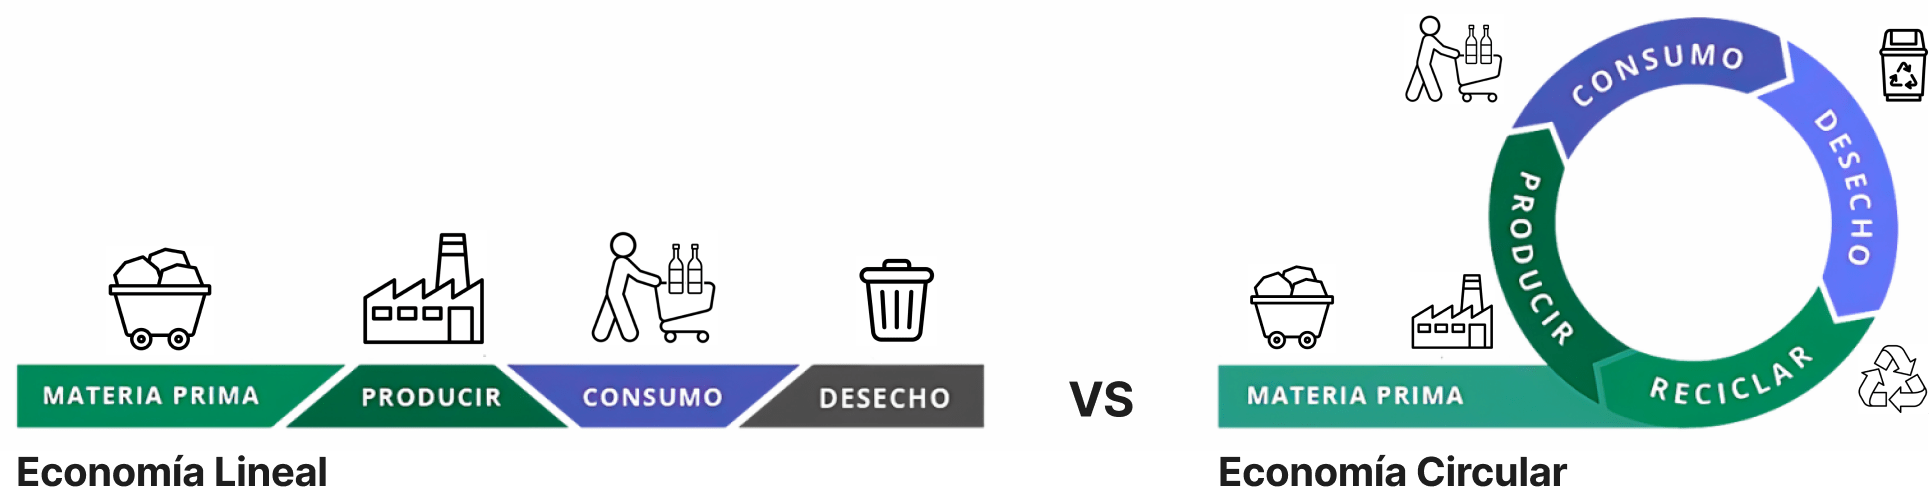
\includegraphics[width=\textwidth]{Figures/circular-linear-economy-comparison.png}
    \caption{Comparación entre la economía lineal y la economía circular}
    \label{fig:circular-linear-economy-comparison}
\end{figure}

En la actualidad existen desafíos culturales, normativos y tecnológicos que dificultan la implementación de la economía circular a gran escala. La transición de los sistemas productivos requiere inversión en infraestructura, marcos regulatorios adecuados y políticas de incentivos claros. Asimismo, implica repensar la educación y la formación de trabajadores para adaptarse a nuevas dinámicas laborales \cite{da2022economia}. En muchos contextos, como América Latina y el Caribe, también se han identificado limitaciones institucionales y de gobierno que deben ser abordadas para permitir una adopción efectiva del modelo \cite{cepal2021economia}. Esta transición ya se encuentra en marcha. Numerosos países y sectores productivos han comenzado a incorporar principios circulares en sus estrategias de desarrollo, en muchos casos impulsados por marcos regulatorios, acuerdos internacionales y metas vinculadas a la sostenibilidad ambiental \cite{da2022economia, cepal2021economia}. En este contexto, las políticas públicas han asumido un rol central como motores de adopción, ofreciendo instrumentos normativos, fiscales y de gobernanza que facilitan la transformación del sistema económico. A continuación, se analizará un conjunto de políticas sustentables relevantes para avanzar hacia una economía más circular .

\subsection{Políticas sustentables}

En el proceso de transición hacia modelos de desarrollo más sostenibles, la Unión Europea ha asumido un rol pionero en la implementación de políticas públicas alineadas con la \gls{economiacircular}. Iniciativas como el Pacto Verde Europeo y la Ley Europea del Clima han consolidado a Europa como un referente global en materia de sustentabilidad ambiental \cite{dormido2022cambio}. Estas políticas no solo promueven la descarbonización de la economía, sino que también introducen principios de circularidad en sectores como la industria, la energía, la movilidad y la gestión de residuos, reconfigurando las cadenas de suministro hacia sistemas más regenerativos, transparentes y trazables.

Sin embargo, el mayor hito internacional en la construcción de una visión compartida sobre sustentabilidad ha sido la adopción de los \acrfull{ods} de Naciones Unidas en 2015. Este conjunto de 17 objetivos interconectados (Figura \ref{fig:ods}), acompañados por 169 metas y más de 230 indicadores, propone una agenda universal que orienta las políticas públicas hacia un desarrollo económico, social y ambiental equilibrado para 2030 \cite{gil2018objetivos}.

\begin{figure}[!tb]
    \centering
    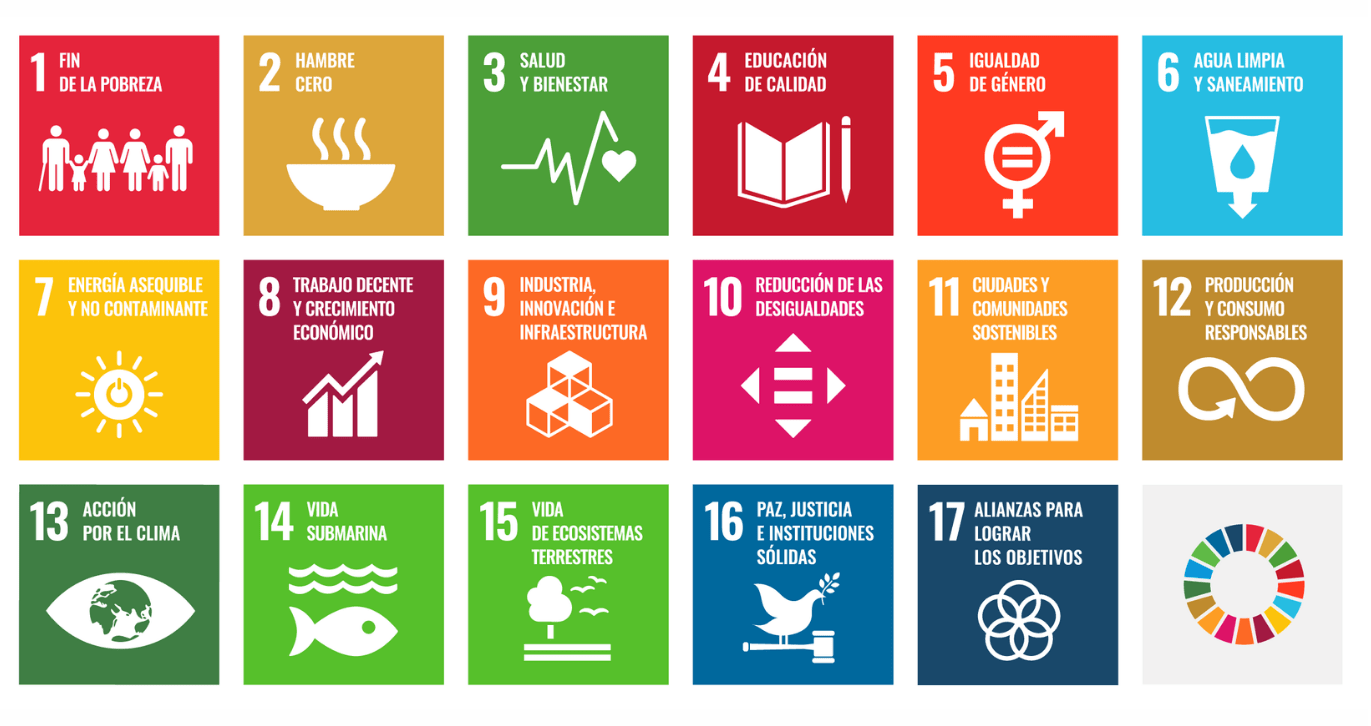
\includegraphics[width=0.8\textwidth]{Figures/ods.png}
    \caption[\acrfull{ods} de Naciones Unidas]{\acrfull{ods} de Naciones Unidas. Fuente: \cite{onu2024ods}}
    \label{fig:ods}
\end{figure}

El objetivo general de los \acrshort{ods} es erradicar la pobreza, proteger el planeta y garantizar la paz y prosperidad para todas las personas. En relación con la economía circular, se identifican un conjunto de objetivos particularmente relevantes que guían tanto los marcos normativos como las estrategias de innovación en producción, consumo y gestión de residuos:

\begin{itemize}
\item \textbf{\acrshort{ods} 7: Energía asequible y no contaminante.}\footnote{\url{https://www.un.org/sustainabledevelopment/es/energy/}} Promueve el acceso universal a fuentes de energía limpias, eficientes y modernas, fundamentales para la transición a una economía circular descarbonizada.
\item \textbf{\acrshort{ods} 11: Ciudades y comunidades sostenibles.}\footnote{\url{https://www.un.org/sustainabledevelopment/es/cities/}} Plantea la necesidad de gestionar de manera integrada los recursos urbanos, incluyendo residuos, infraestructura y movilidad, en articulación con una trazabilidad eficiente de los flujos materiales.
\item \textbf{\acrshort{ods} 12: Producción y consumo responsables.}\footnote{\url{https://www.un.org/sustainabledevelopment/es/sustainable-consumption-production/}} Es el núcleo del paradigma circular, impulsando el diseño sostenible de productos, el uso eficiente de recursos, la minimización de residuos y la promoción de modelos de cadena de suministro regenerativos.
\item \textbf{\acrshort{ods} 13: Acción por el clima.}\footnote{\url{https://www.un.org/sustainabledevelopment/es/climate-change-2/}} Vincula la circularidad con la reducción de emisiones y la adaptación al cambio climático, incentivando políticas que rediseñen los sistemas productivos de alto impacto ambiental.
\end{itemize}

Los \acrshort{ods} han generado un marco de referencia común que ha influido fuertemente en las agendas de \gls{sostenibilidad} a nivel global, incluyendo América Latina \cite{sostenible2021argentina}. Aunque en la región la adopción de políticas circulares aún es incipiente en comparación con Europa, se observan avances significativos en la última década. Por ejemplo, varios países han comenzado a incorporar la responsabilidad extendida del productor, prohibiciones de plásticos de un solo uso y normativas orientadas a la reutilización y reciclado de materiales \cite{cepal2021economia}. Estas políticas buscan reestructurar las cadenas de valor y fomentar prácticas productivas y logísticas compatibles con los principios de circularidad.

En Argentina, la Estrategia Nacional de Consumo y Producción Sostenibles se destaca como el instrumento central para avanzar hacia la economía circular. La estrategia integra medidas normativas, educativas, tecnológicas y financieras, orientadas a fortalecer la sostenibilidad en toda la cadena de producción y consumo. Promueve activamente el uso de tecnologías limpias, la gestión sostenible de recursos y la incorporación de criterios ambientales en compras públicas, reconociendo el rol central de la trazabilidad como mecanismo para garantizar la transparencia, eficiencia y cumplimiento normativo en los sistemas productivos y sus cadenas de suministro \cite{sostenible2021argentina}.

Estas políticas dejan ver que la transformación hacia una economía circular no puede pensarse sin una reconfiguración de las cadenas de suministro, que constituyen la columna vertebral de los sistemas productivos. La implementación de políticas sustentables, tanto en Europa como en América Latina, ha puesto en evidencia la necesidad de contar con mecanismos que permitan monitorear, verificar y optimizar el flujo de materiales a lo largo de todo el ciclo de vida de los productos. En la siguiente sección se abordará con mayor detalle cómo se articula esta relación entre cadenas de suministro y \gls{trazabilidad}, y cuál es su rol estratégico en la transición hacia un modelo económico circular.

\subsection{Cadena de suministro}
\label{sec:supply-chain}

En el contexto de la \gls{economiacircular}, la \gls{cadenadesuministro} asume una nueva lógica de funcionamiento. Pasa de ser una secuencia finita de pasos que culminan con el consumo y disposición del producto, a transformarse en un sistema cíclico, en el cual los productos son diseñados para permanecer en uso el mayor tiempo posible y ser reutilizados, reacondicionados o reciclados \cite{cerda2016economia}. 

La cadena de suministro constituye el entramado logístico, operativo y estratégico que permite el flujo de materiales, información y recursos desde la extracción de materias primas hasta la llegada de un producto al consumidor final. La Figura \ref{fig:supply-chain} permite visualizar este sistema complejo que involucra múltiples etapas y diferentes actores: proveedores, fabricantes, distribuidores, comerciantes, consumidores y, en el caso del modelo circular, gestores de residuos y reguladores. Su objetivo es garantizar que los bienes y servicios se produzcan y entreguen de manera eficiente, segura y rentable \cite{rodriguez2023modelamiento}.

\begin{figure}[!tb]
    \centering
    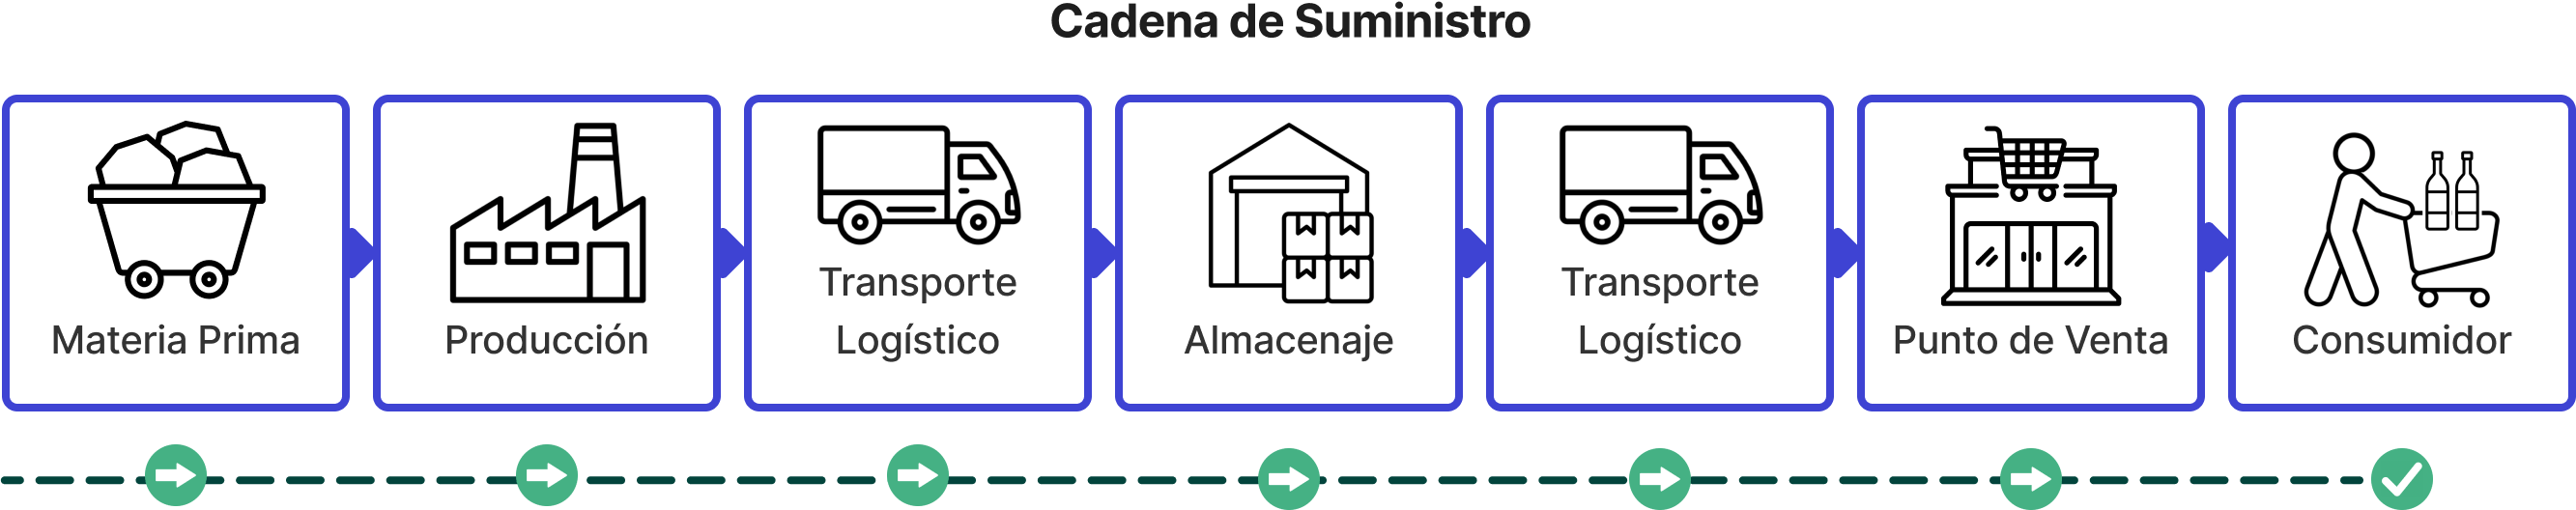
\includegraphics[width=\textwidth]{Figures/supply-chain.png}
    \caption{Componentes de una cadena de suministro}
    \label{fig:supply-chain}
\end{figure}

A lo largo de los años, las cadenas de suministro se han establecido para maximizar la eficiencia y reducir costos en la producción de productos. Con este objetivo claro, es que se ha dividido el proceso en etapas y se aplican herramientas, procesos y tecnologías diversas para optimizar cada una de ellas, desde la adquisición de materias primas hasta la distribución final. Sin embargo, la maximización de la eficiencia en este modelo lineal, sin preocuparse por el destino del producto luego de su uso, ha generado efectos secundarios adversos en el medioambiente que, como ya se mencionó, han llevado a la necesidad de un modelo sostenible en el tiempo \cite{espanacircular2030}.

Para diseñar una cadena de suministro circular, la \gls{trazabilidad} se posiciona como la herramienta que permite mantener y mejorar la eficiencia y costos, mientras que permite incorporar al final de la cadena las etapas de disposición, reciclaje y reutilización de materiales. La trazabilidad es la capacidad de seguir el recorrido completo de un producto, material o componente a lo largo de toda la cadena de suministro, desde su origen hasta su destino final. Su objetivo principal es reconstruir el historial de producción, transformación y movimiento de un bien, permitiendo conocer su composición, ubicación, responsables y condiciones de manejo en cada etapa del proceso \cite{bartolomeo2020introduccion}. Por ejemplo, aplicando trazabilidad en la producción de vino se puede conocer la parcela de origen de la uva, la fecha de la vendimia y el proceso de añejamiento, permitiendo al consumidor verificar su autenticidad y al productor identificar rápidamente cualquier problema en un lote. Otro ejemplo frecuente es la trazabilidad de residuos peligrosos, que permite verificar que la disposición final del residuo se hizo correctamente para evitar riesgos de salud o ambientales. La información permite verificar la autenticidad del producto, asegurar estándares de calidad, cumplimiento normativo, eficiencia operativa y \gls{sostenibilidad} ambiental. Procesos de trazabilidad establecidos permiten también identificar riesgos y oportunidades de mejora en la cadena, permitiendo optimizar la logística, reducir costos y riesgos asociados a errores, fraudes o contaminaciones, y mejorar la capacidad de respuesta ante incidentes o fallas. En la cadena de suministro, la trazabilidad se aplica de forma transversal (Figura \ref{fig:supply-chain-traceability}), es decir, atraviesa e interconecta todas las fases del ciclo: desde el diseño y la fabricación, hasta la distribución, el consumo, la gestión de residuos y el reciclaje \cite{cepal2021economia}.

\begin{figure}[!tb]
    \centering
    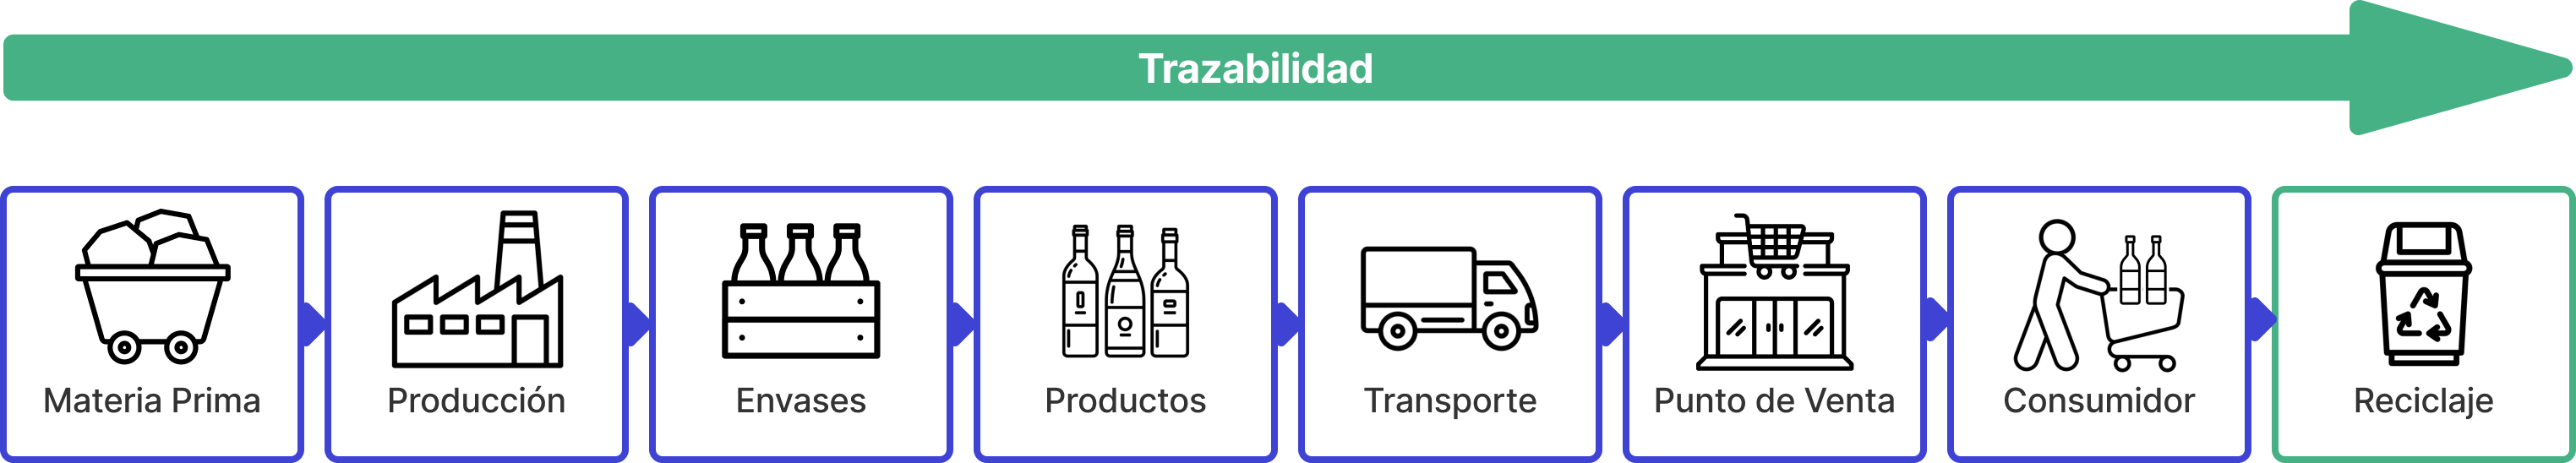
\includegraphics[width=\textwidth]{Figures/supply-chain-traceability.png}
    \caption{Ejemplo de trazabilidad como herramienta transversal en la cadena de suministro de envases de vino}
    \label{fig:supply-chain-traceability}
\end{figure}

No obstante, la implementación de trazabilidad en la cadena de suministro conlleva desafíos importantes. Las cadenas de suministro tradicionales suelen estar fragmentadas y utilizar sistemas de información heterogéneos o poco interoperables \cite{torres2022tendencias}. Muchos registros todavía se realizan en papel o en bases de datos centralizadas, lo que aumenta la vulnerabilidad frente a errores humanos, pérdidas de datos o manipulaciones \cite{bartolomeo2020introduccion}. Además, la ausencia de estándares unificados y la reticencia a compartir datos entre organizaciones limitan la visibilidad total del flujo de productos y materiales. Para abordar estos desafíos, se ha desarrollado un conjunto de tecnologías que fortalecen los sistemas de trazabilidad. Entre las más utilizadas se encuentran los códigos de barras y las etiquetas \acrshort{rfid}, que permiten la identificación automática de productos mediante etiquetas físicas; los sensores \acrshort{iot}, que capturan datos en tiempo real sobre condiciones ambientales o de transporte; los sistemas ERP y de gestión logística digitales, que centralizan y organizan la información operativa; y, más recientemente, la tecnología blockchain se está posicionando como solución para unificar a todos los actores de la cadena aportando una nueva capa de transparencia entre etapas y resolviendo problemas de confianza entre los diferentes actores \cite{wong2024enhancing}.

La tecnología blockchain permite registrar cada transacción o evento de la cadena de suministro en una \gls{basededatos} digital descentralizada e inalterable. Esto garantiza que todos los actores tengan acceso a un historial común y verificable, reduciendo la necesidad de intermediarios y auditores externos. Combinando \glspl{contratointeligente} y plataformas de análisis de datos, la trazabilidad basada en blockchain permite no solo conocer lo que ocurrió, sino también automatizar respuestas ante condiciones predefinidas, reduciendo los tiempos de reacción y aumentando la confianza entre las partes \cite{wong2024enhancing}. El uso de blockchain en este contexto aporta un aumento significativo en la seguridad, transparencia, precisión de datos, eficiencia, responsabilidad y confianza entre actores. Esta tecnología ya se está utilizando para trazabilidad en diversos sectores como la agricultura, alimentos, industria textil y medioambiente. Por ejemplo, en el sector alimenticio, impulsa el valor percibido del producto y la calidad, además de fortalecer la confianza entre las partes interesadas. Para el sector industrial, su uso se enfoca en la planeación y el intercambio de información para una mayor \gls{sostenibilidad}. Además, es posible combinar tecnología Blockchain con \acrshort{iot} y otros sistemas digitales ya implementados en la cadena de suministro. Esta combinación puede proporcionar soluciones aún más eficientes para la cadena de suministro, automatizando la recopilación de datos confiables y aumentando los beneficios para las partes interesadas \cite{wong2024enhancing}. A continuación, se explorará cómo se articula el proceso de producción y reciclaje en la economía circular, y cómo la trazabilidad digital puede potenciar este ciclo.

\subsection{Proceso de producción y reciclaje en la economía circular}

En el marco de la \gls{economiacircular}, los procesos de producción y reciclaje dejan de concebirse como etapas aisladas y unidireccionales para integrarse en un sistema dinámico y regenerativo. Como puede observarse en la Figura \ref{fig:circular-economy-stages}, la cadena de suministro del proceso productivo incluye la gestión de residuos y la reinserción de materiales reciclados en nuevos ciclos productivos \cite{cepal2021economia}.

\begin{figure}[!b]
    \centering
    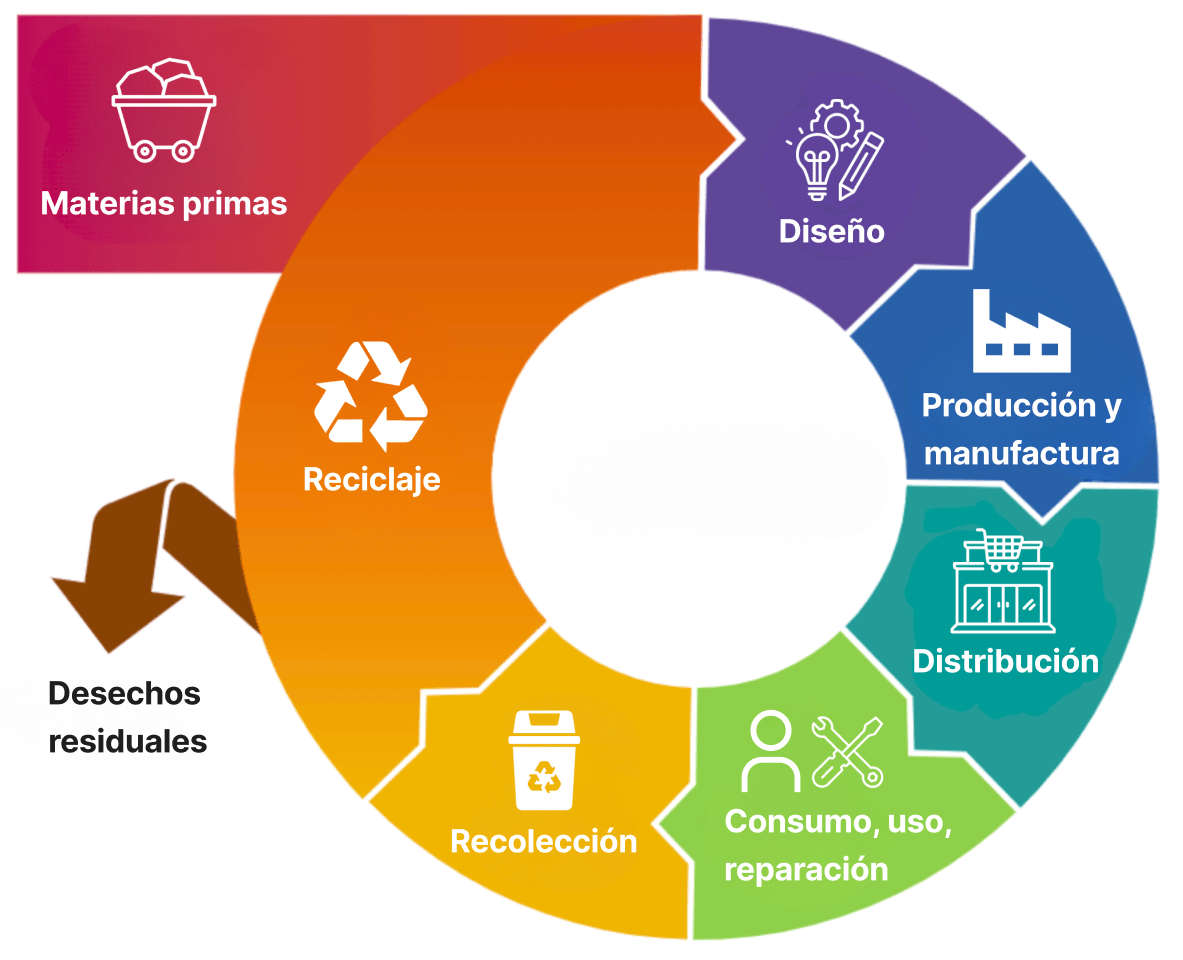
\includegraphics[width=0.5\textwidth]{Figures/circular-economy-stages.png}
    \caption{Ciclo productivo de la economía circular}
    \label{fig:circular-economy-stages}
\end{figure}

El proceso de producción comienza propiamente con la etapa de diseño, donde se decide la composición de los productos considerando criterios de ecoeficiencia, reutilización y reciclabilidad. Aquí intervienen diseñadores, ingenieros y proveedores de materias primas, quienes priorizan materiales reciclados o de bajo impacto ambiental. A continuación, durante la fabricación, los procesos industriales buscan reducir el uso de recursos y minimizar las emisiones, integrando tecnologías limpias y eficientes \cite{espanacircular2030}. En esta fase, los productos terminados o semielaborados quedan registrados con información detallada sobre su origen, composición y trazabilidad, lo cual permite una futura gestión más eficiente de su reciclaje. Tras su elaboración, los productos son distribuidos a través de canales logísticos que buscan optimizar los costos e impacto ambiental del transporte y almacenamiento.

Una vez que los productos son utilizados por los consumidores, comienza el ciclo inverso de valorización. Cuando estos artículos llegan al fin de su vida útil (y ya no pueden ser reutilizados), se convierten en residuos que deben ser recolectados, transportados, clasificados y reciclados o reacondicionados. Este proceso, conocido de forma genérica como ``reciclaje'' (sin distinguir si el destino final es reacondicionamiento o reciclaje), involucra a recolectores, centros de acopio, plantas de tratamiento, recicladores industriales y fabricantes secundarios \cite{cepal2021economia}. Durante la recolección, tecnologías como sensores \acrshort{iot}, lectores de códigos \acrshort{qr} o etiquetas \acrshort{rfid} permiten registrar información sobre la identidad del recolector, la cantidad, el tipo y las condiciones del residuo. Esta información permite monitorear flujos de materiales y brindar transparencia en la cadena \cite{wong2024enhancing}. En el primer paso del proceso de reciclaje, los residuos son transportados a instalaciones donde se clasifican y segregan según su tipo y calidad. Este paso es fundamental para evitar contaminaciones cruzadas entre materiales distintos y asegurar un reciclaje efectivo. Posteriormente, los materiales seleccionados se someten a procesos de reciclaje o reacondicionamiento, reincorporándolos al sistema productivo como insumos o productos reutilizables. En todo este proceso, tecnologías como blockchain pueden documentar cada transacción o transformación del material, documentando la integridad del proceso y fomentando la confianza entre los actores \cite{wong2024enhancing}.

Baralla et al. \cite{baralla2023waste}, en su trabajo, ilustran mediante la Figura \ref{fig:baralla-model-1} las distintas aplicaciones posibles de la tecnología blockchain en cada etapa del ciclo completo de economía circular. En este sistema esquemático, la tecnología blockchain conecta las etapas en un flujo de información unificado, formando un sistema de trazabilidad digital que permite el seguimiento de los materiales desde su origen hasta su reincorporación al sistema o disposición final.

\begin{figure}[!tb]
    \centering
    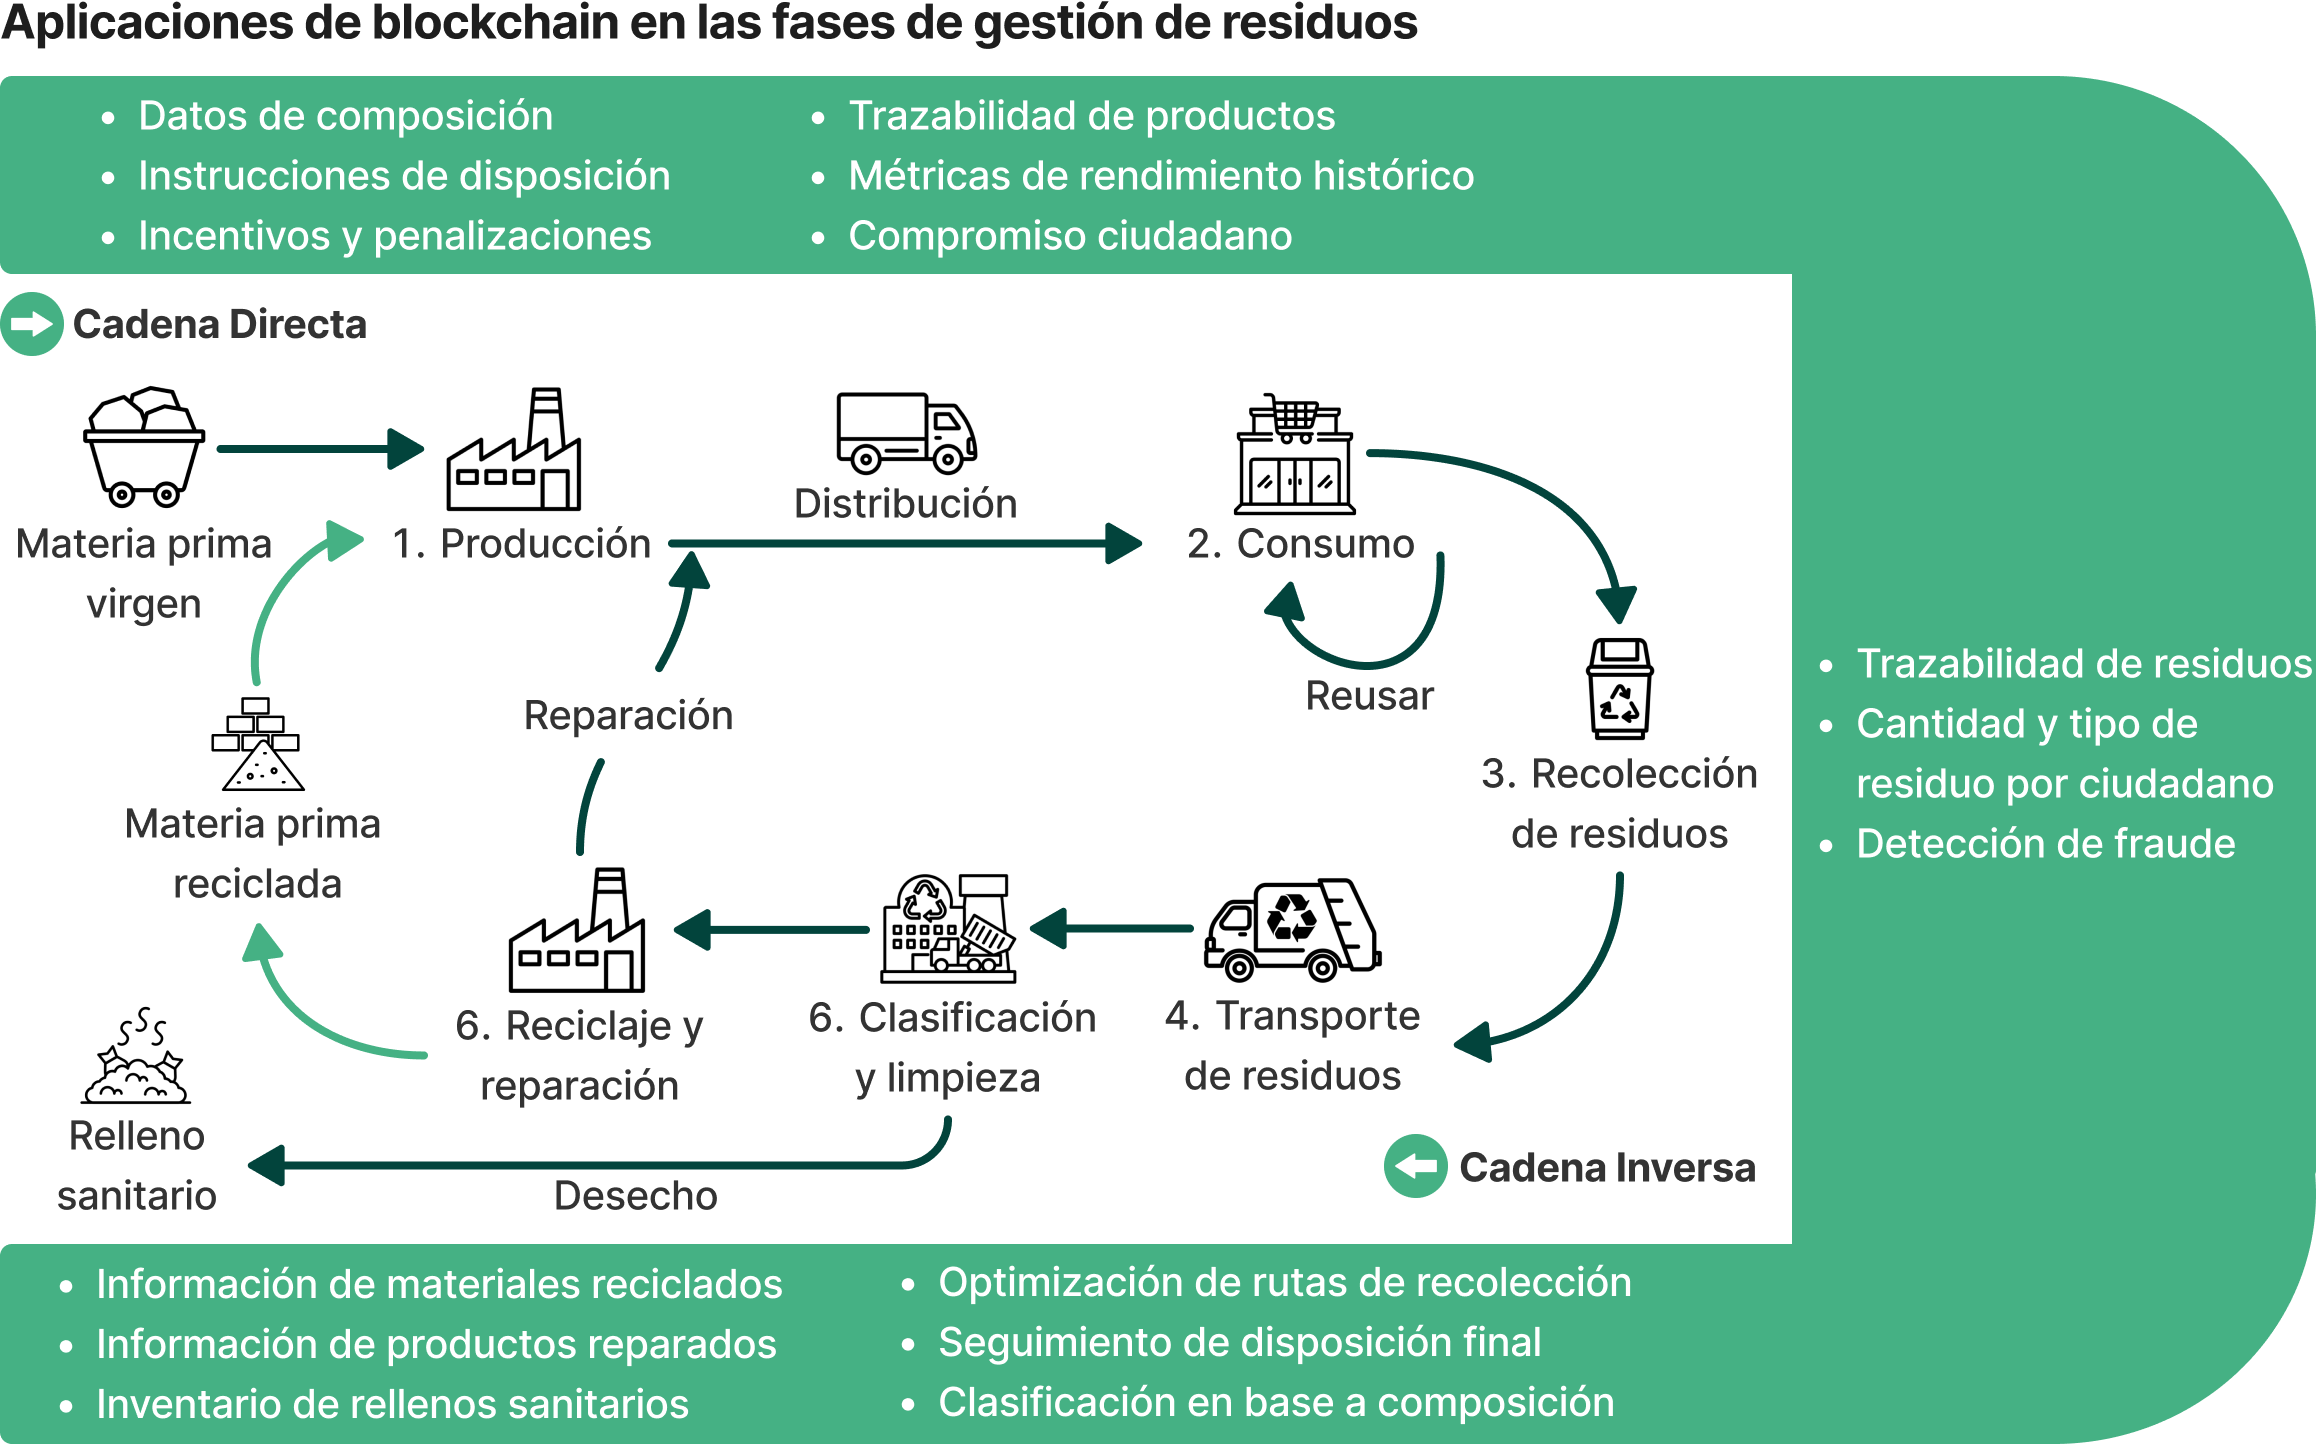
\includegraphics[width=\textwidth]{Figures/baralla-model-1.png}
    \caption[Usos de la tecnología blockchain en la economía circular]{Usos de la tecnología blockchain en las etapas de la economía circular \cite{baralla2023waste}}
    \label{fig:baralla-model-1}
\end{figure}

El proceso de reciclaje varía en complejidad dependiendo del material. Existen diversos materiales reciclables, cada uno con características particulares. El papel y cartón son ampliamente reciclados y fáciles de recolectar, mientras que los metales (como el aluminio, el acero o el cobre) conservan sus propiedades tras múltiples ciclos \cite{cepal2021economia}. Los residuos electrónicos presentan un alto valor por su contenido en metales preciosos, aunque requieren procesos especializados para su desmontaje. Los plásticos representan un desafío por su heterogeneidad, pero pueden reciclarse eficientemente si se rediseñan los envases y se simplifican sus composiciones. Los residuos orgánicos son compostables o pueden aprovecharse energéticamente en caso de no mezclarse con residuos no reciclables. Finalmente, el vidrio destaca como el material circular por excelencia: puede reciclarse infinitas veces sin perder calidad, su estructura es químicamente estable, y su reciclaje requiere menos energía que su producción original \cite{verallia2022whitebook}. Estas cualidades lo convierten en un insumo ideal para sistemas de economía circular bien diseñados.

\subsection{Cadena de suministro del vidrio}
\label{sec:glass-supply-chain}

El vidrio es uno de los materiales más representativos de la \gls{economiacircular} por su capacidad única de ser reciclado indefinidamente sin perder calidad \cite{verallia2022whitebook}. Esta propiedad lo convierte en un recurso estratégico para reducir la demanda de materias primas vírgenes, minimizar residuos y disminuir la huella de carbono asociada a la producción industrial. A diferencia de otros materiales cuyo reciclaje implica degradación, el vidrio conserva íntegramente sus características físicas y químicas, permitiendo su reintegración al ciclo productivo tantas veces como sea necesario.

\begin{figure}[!b]
    \centering
    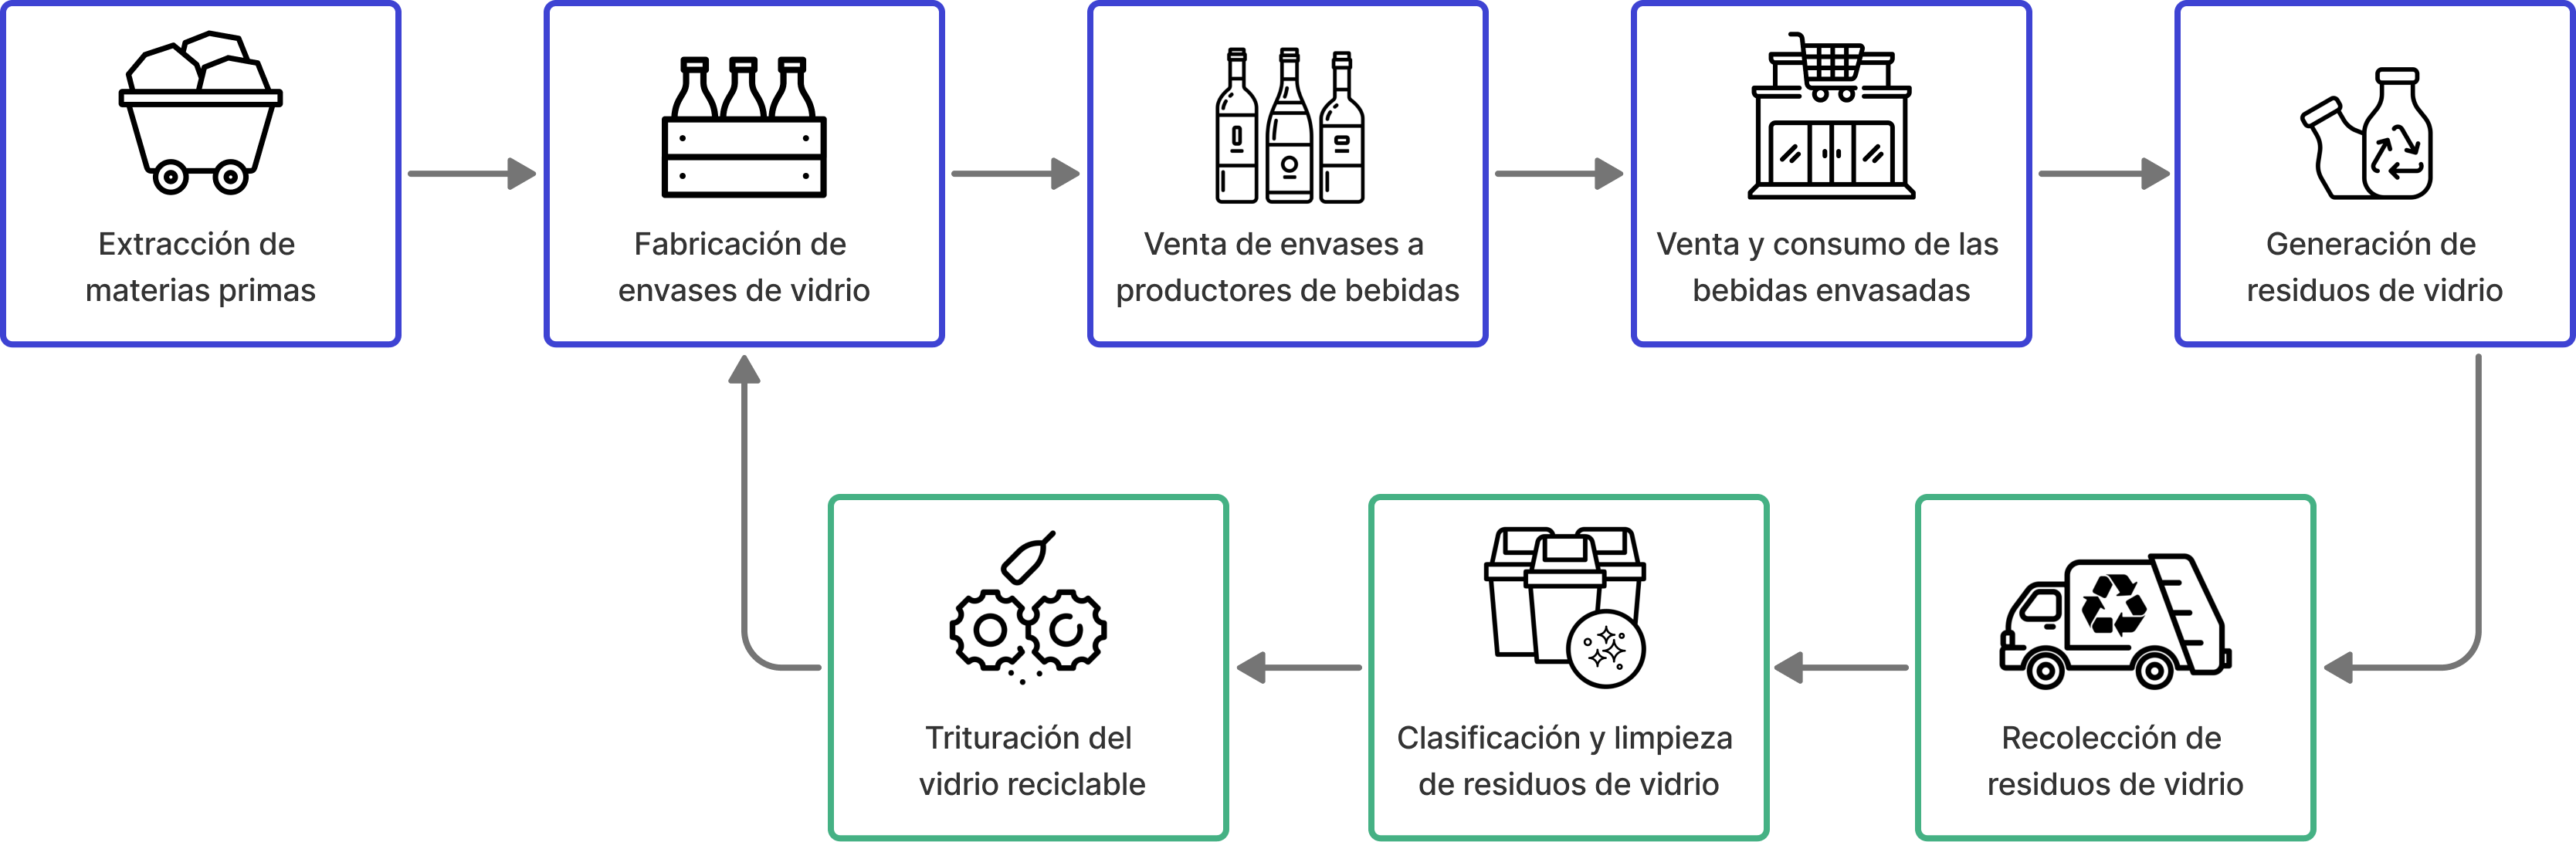
\includegraphics[width=\textwidth]{Figures/glass-lifecycle.png}
    \caption{Ciclo de vida de envases de vidrio en un modelo de economía circular}
    \label{fig:glass-lifecycle}
\end{figure}

En la Figura \ref{fig:glass-lifecycle} se muestra el ciclo de vida del vidrio en un modelo de economía circular, que abarca desde la extracción de materias primas hasta su reincorporación como materia prima en nuevos productos, ejemplificando el caso de los envases de vidrio \cite{prodvidrio2024verallia}. El proceso comienza con el diseño del producto, etapa clave para asegurar su durabilidad, reutilización y posterior reciclabilidad. Por ejemplo, en la producción de envases de vidrio, en esta etapa se deciden aspectos como color, forma y composición del envase para optimizar durabilidad, reciclabilidad y aspectos estéticos. Luego del diseño, sigue la producción industrial, donde se funden arena, sosa y caliza a altas temperaturas, frecuentemente combinadas con calcín (vidrio reciclado triturado) para reducir el consumo energético y demanda de materiales vírgenes. La especial reciclabilidad del vidrio se hace visible en esta etapa, ya que la calidad del vidrio resultante es la misma sin importar la proporción de calcín y de materiales vírgenes utilizados (característica que, por ejemplo, no es igual para el plástico), por lo que los productores de vidrio no encuentran pérdidas potenciales al utilizar materiales reciclados. Luego, los envases fabricados son distribuidos, utilizados para embotellar bebidas (por ejemplo, vino) y adquiridos por los consumidores, quienes (luego de consumir su contenido) pueden reutilizarlos, descartarlos (como basura común) o ingresarlos a circuitos de reciclaje. Para el correcto reciclaje del vidrio (y otros materiales) es importante el circuito de recolección diferenciada, que evita que el vidrio reciclable se mezcle con otros materiales que lo contaminen e imposibiliten su reciclaje. Los residuos de vidrio son recolectados por empresas especializadas o por los propios consumidores, quienes pueden depositarlos en contenedores específicos para su posterior tratamiento.
Una vez recolectado, el vidrio es transportado a plantas de reciclaje donde se clasifica. En la clasificación se separa al vidrio de otros materiales reciclables que puedan haber sido mezclados y se separan los distintos tipos de vidrio (por ejemplo, por color), ya que algunas características, como el color y la composición química, son relevantes para el posterior uso del vidrio reciclado. Luego, el vidrio es triturado y limpiado para eliminar impurezas, como etiquetas o restos de alimentos, dando como resultado lo que se conoce como calcín. Esta etapa es crucial, ya que la pureza del material reciclado influye directamente en la calidad del vidrio producido. Finalmente, el calcín se funde nuevamente y se convierte en materia prima para nuevos envases, cerrando así el ciclo de vida del vidrio. Este proceso de reciclaje puede repetirse indefinidamente, lo que lo convierte en un modelo ejemplar de economía circular.

La \gls{cadenadesuministro} y reciclaje de envases de vidrio tiene una importancia estratégica en la provincia de Mendoza, por su estrecha vinculación con la industria vitivinícola, uno de los principales motores económicos de la región. La provincia cuenta con una única empresa que produce y recicla envases de vidrio a escala industrial: Verallia \footnote{\url{https://ar.verallia.com/}}. Esta compañía internacional cubre la totalidad de la demanda local de botellas y frascos, fabricando envases para vinos, espumantes, cervezas, licores y alimentos. El proceso de producción en Verallia incluye desde la selección y mezcla de materias primas hasta la formación, inspección y distribución de los envases, con la integración progresiva de vidrio reciclado como parte del insumo.

Verallia ha reconocido públicamente que la mayor dificultad de su industria es la elevada emisión de dióxido de carbono, por lo que ha adoptado una estrategia dual orientada a optimizar el reciclaje y fomentar la reutilización del vidrio. Bajo esta lógica, ha desarrollado el programa ``Vidrio, una acción transparente'' en alianza con el Gobierno de Mendoza, mediante el cual se promueve la recolección de envases descartados, destinando los ingresos generados al apoyo de organizaciones benéficas. Esta iniciativa, aunque aún incipiente, representa un esfuerzo por avanzar hacia una cadena de suministro más circular y socialmente responsable en la provincia.

Sin embargo, el reciclaje de vidrio en Mendoza enfrenta desafíos estructurales. La tasa de recuperación aún es baja, las métricas oficiales son escasas y las políticas de incentivo son limitadas. La logística de recolección depende en gran medida de la voluntad ciudadana y carece de sistemas obligatorios o premiantes que aseguren su masividad. En este contexto, el rol de actores industriales como Verallia resulta central para impulsar transformaciones sostenibles en la cadena del vidrio, tanto mediante la innovación tecnológica como a través de la articulación público-privada.

Más allá del caso mendocino, el vidrio sigue siendo uno de los materiales más valiosos dentro de una economía circular bien implementada. Su durabilidad, estabilidad química, transparencia y capacidad de reciclaje total lo convierten en un insumo ideal para cerrar ciclos productivos sin pérdidas de calidad ni de valor. Avanzar hacia una cadena del vidrio plenamente circular requiere optimizar cada etapa, desde el diseño y la fabricación hasta la trazabilidad del reciclaje, consolidando sistemas logísticos eficientes, ciudadanos comprometidos y políticas públicas robustas que garanticen su \gls{sostenibilidad} a largo plazo. En este contexto, la incorporación de sistemas basados en tecnología blockchain ofrece la posibilidad de reforzar la trazabilidad a lo largo de toda la cadena de suministro, facilitando un uso más eficiente y seguro de la información en cada etapa. Esta integración no solo optimiza la operación de cada parte involucrada, sino que también impulsa la adopción de prácticas de economía circular y el uso de blockchain en la región. Tomando esta iniciativa como base para el proyecto, a continuación se detallan proyectos y trabajos previos que han explorado la trazabilidad y el reciclaje de vidrio, así como otras iniciativas vinculadas a la economía circular y la sostenibilidad, las cuales aportan soluciones innovadoras para la gestión de residuos y la promoción de prácticas responsables en la cadena de suministro.

\section{Proyectos y Trabajos Relacionados}
\label{sec:related-work}

La tecnología blockchain se ha posicionado como una herramienta poderosa para mejorar la \gls{trazabilidad} en cadenas de suministro, ofreciendo registros inmutables y transparentes que permiten rastrear el movimiento de productos desde su origen hasta el consumidor final. Esta característica fortalece la confianza entre los actores y favorece la \gls{economiacircular}, al garantizar la autenticidad e integridad de la información. Numerosos proyectos, tanto académicos como comerciales, han explorado su aplicación en la gestión de residuos y en la trazabilidad de materiales. A continuación, se presentan casos representativos con sus características, beneficios y limitaciones, a fin de identificar lecciones aplicables al desarrollo de un sistema de trazabilidad para el vidrio.

En el ámbito académico, Baralla et al. en su trabajo ``Waste Management: A Comprehensive State of the Art about the Rise of Blockchain Technology'' \cite{baralla2023waste} exploran la trazabilidad de residuos, prevención de fraude e incentivos mediante \glspl{contratointeligente}. El modelo planteado (Figura \ref{fig:baralla-model-1}) permite gestionar tanto la cadena directa (producción y consumo) como la inversa (reciclaje), pero señala la necesidad de enfocarse en categorías específicas de residuos y advierte sobre desafíos de escalabilidad, privacidad y rendimiento en blockchains públicas. A su vez, Rahman et al. \cite{rahman2025traceable} profundizan en cómo la tecnología blockchain permite abordar las vulnerabilidades de los sistemas de gestión de residuos tradicionales que facilita el fraude, como la falta de transparencia. En este trabajo se introduce el concepto de ``Pasaporte Digital de Producto'', un registro digital en la blockchain que documenta información clave del producto a lo largo de su existencia, desde la composición de sus materiales y su origen, hasta su historial de uso y sus procesos de reciclaje asociados al final de su vida útil. Este enfoque, según los autores, se potencia al integrarse con tecnologías \acrshort{iot}, donde los sensores pueden recolectar datos en tiempo real (por ejemplo, niveles de llenado en contenedores) para que sean registrados de forma segura en la blockchain, optimizando así la logística y la eficiencia del sistema.

Dando un paso más allá de la revisión conceptual, Bathaei et al. \cite{bathaei2025blockchain} proponen un marco orientado a la toma de decisiones para que las organizaciones puedan evaluar y priorizar estratégicamente las diferentes soluciones de blockchain para la gestión de residuos. Su principal aporte es la aplicación de una metodología mixta que combina el conocimiento de un panel de expertos con herramientas de decisión multicriterio como el \textit{Best-Worst Method}. A través de este método, el estudio identifica y cuantifica la importancia relativa de los criterios de evaluación, concluyendo que la trazabilidad del material y el cumplimiento regulatorio son los factores más críticos para el éxito de la implementación de blockchain en la gestión de residuos. Este enfoque metodológico traslada el debate desde el potencial teórico de la tecnología hacia una guía práctica y validada empíricamente para la toma de decisiones de inversión y desarrollo en la economía circular.

Otro caso académico es el Modelo ZERO de Sandhiya et al. \cite{sandhiya2020investigating} para reciclaje de plásticos, que integra códigos \acrshort{qr}, \acrshort{iot} y blockchain para proveer un sistema de trazabilidad inmutable y brindar incentivos para reciclar a los consumidores. En este modelo, cada producto lleva un \acrshort{qr} único grabado molecularmente, evitando manipulaciones, y se utilizan ``bines inteligentes'' que aceptan solo plásticos válidos, con verificación y clasificación automática en máquinas de reciclaje. El modelo ofrece incentivos monetarios a los consumidores y busca mejorar calidad, transparencia y costos del reciclaje. De forma complementaria, Bhubalan et al. \cite{bhubalan2022blockchain} proponen integrar blockchain con marcadores moleculares para rediseñar químicamente plásticos y lograr un reciclaje cerrado. Aunque reconocen su potencial técnico, cuestionan la rentabilidad para plásticos de un solo uso debido a los altos costos de implementación. Estos trabajos demuestran que blockchain puede integrarse con tecnologías de identificación física para reforzar la trazabilidad, pero el nivel de infraestructura requerida puede limitar su adopción en contextos con recursos más restringidos, como el reciclaje de vidrio en entornos municipales o regionales. A su vez, la lógica de incentivar al consumidor mediante un mecanismo verificable y confiable, presente en el Modelo ZERO, encuentra un ejemplo real y ampliamente adoptado en el sistema \acrfull{drs} de Alemania \cite{picuno2025potential}. Este sistema de \acrshort{drs} no emplea blockchain, pero materializa en la práctica el principio fundamental de estos trabajos: ofrecer una recompensa directa y comprobable para asegurar que el material reciclable retorne a la cadena de valor.

La efectividad de este enfoque se confirma con múltiples experiencias regionales e internacionales, que demuestran que la incorporación de incentivos tangibles es un factor clave para fomentar hábitos de reciclaje en los consumidores e impulsar el desarrollo de una economía circular. En España, Reciclos \cite{reciclos2024} ofrece recompensas por el reciclaje de latas y botellas. En Argentina, Colmena \cite{colmena2024} premia a los usuarios con la \gls{criptomoneda} JellyCoin, mientras que Greenly Points \cite{greenlypoints2024} en Mendoza y Reciqlo en Buenos Aires \cite{innovar2024vidrio} otorgan puntos canjeables por beneficios locales al entregar residuos reciclables en puntos verdes, y este último centra su actividad exclusivamente en la recolección y el reciclaje de vidrio. A nivel global, Plastic Bank en Canadá utiliza la tecnología blockchain para ofrecer criptomonedas como incentivo a los recolectores de plástico en regiones empobrecidas, demostrando cómo las recompensas digitales pueden impulsar la participación y aumentar la transparencia en el flujo de residuos. Estas experiencias subrayan que, al ofrecer valor a cambio del material reciclable, se logra una mayor involucración ciudadana y se contribuye de manera significativa a cerrar los ciclos de vida de los productos.

Asimismo, existen múltiples soluciones comerciales que aplican blockchain para trazabilidad en cadenas de suministro. Entre ellas se destaca Signeblock (España) \cite{signeblock2024} con su producto Gouze, que permite registrar cada paso de los procesos productivos y de distribución en blockchain, ofreciendo acceso personalizado a la información mediante un gestor documental unificado. Incorpora digitalización y notarización de procesos, certificación blockchain para garantizar inalterabilidad y códigos \acrshort{qr} para compartir información del proceso con consumidores. Sus principales limitaciones se relacionan con la interoperabilidad con sistemas existentes y la resistencia organizacional a compartir datos entre actores. Otra solución relevante es Circularise (Países Bajos) \cite{circularise2024}, plataforma que ofrece pasaportes digitales de productos para trazabilidad de extremo a extremo y el intercambio seguro de datos. Para cada producto registra origen, composición y datos ambientales respaldados por blockchain, facilitando cálculo de huella de carbono. Integra con sistemas ERP y promueve un enfoque abierto e interoperable, utilizando una blockchain pública descentralizada para asegurar credibilidad. Por su parte, Circulor (Reino Unido) \cite{circulor2024} es una plataforma que proporciona trazabilidad completa desde la fuente hasta el consumidor final, ayudando a demostrar procedencia responsable, reducir emisiones y gestionar riesgos. Se integra con plataformas empresariales mediante \acrshortpl{api}, rastrea materias primas y controla el flujo de materiales en la producción. En conjunto, estas plataformas evidencian la viabilidad de blockchain para trazabilidad industrial a gran escala, integrando datos ambientales y de origen. No obstante, su enfoque en cadenas de alto valor agregado plantea dudas sobre su adaptación a cadenas de reciclaje de vidrio con márgenes de ganancia reducidos y mayor fragmentación de actores.

Los proyectos y modelos analizados evidencian el vasto potencial de la tecnología blockchain para transformar la gestión de residuos y las cadenas de suministro hacia modelos más sostenibles y circulares. Desde sistemas de incentivos simples hasta plataformas complejas de trazabilidad de extremo a extremo, la inmutabilidad, transparencia y descentralización de blockchain ofrecen soluciones prometedoras. No obstante, se identifican puntos débiles recurrentes en su aplicación actual, que incluyen la necesidad de un mayor desarrollo técnico y madurez de la tecnología, la superación de barreras organizacionales (como la reticencia a compartir datos), los altos costos de implementación inicial, problemas de escalabilidad en redes públicas y el consumo energético en ciertos algoritmos de consenso, así como la aún incipiente regulación y falta de estándares comunes. Es en este contexto de oportunidades donde se posiciona el presente trabajo de tesis. A pesar de los avances y el reconocimiento de la importancia del reciclaje de vidrio, especialmente en regiones como Mendoza, con una fuerte industria vitivinícola, se observa una fuerte desconexión entre los actores de la \gls{cadenadesuministro}, baja tasa de recuperación (con escasez de métricas oficiales) y débiles políticas de incentivos. Los programas existentes en Argentina, si bien son un paso adelante, aún carecen de mecanismos obligatorios o premiantes que aseguren la masividad de la recolección diferenciada y no garantizan por sí mismos el reciclaje efectivo del material.

Este trabajo busca abordar estas brechas mediante el desarrollo de un prototipo de sistema de trazabilidad del vidrio basado en tecnología blockchain. Enfocado específicamente en la cadena de suministro del vidrio en el contexto mendocino, con el objetivo de integrar a todos los actores del proceso, desde la producción hasta su reintroducción en la cadena de valor. Este sistema se propone permitir el registro y verificación de cada etapa del ciclo de vida del vidrio, mientras que, a su vez, busca superar las limitaciones identificadas en los proyectos preexistentes al ofrecer una solución que facilite la valorización del vidrio, promoviendo una economía circular más transparente, eficiente y sostenible en la región. En este trabajo se hace énfasis en la usabilidad, la integración de datos relevantes y la demostración de los beneficios tangibles para todos los participantes de la cadena.
